\chapter{Variable selection pressure}
In the original paper, Fernando et al. used a tournament search algorithm for optimizing the modules used for a given task. This algorithm was selected on the basis that it fills the role of simplest possible 'agent' for path-selection, one which can be considered a unit of evolution.  The tournament implementation fits this description as a 'unit' because of the tournament size used. Within one generation, the total change in the population is one genotype being replaced with another from the same population and subjected to mutation under some probability. Building on the previous set of experiments where the conclusion can take form as an argument in favour of a high exploration rate during path-search, we would expect a tournament of size two to yield modules with high transferability and a high number of reuse. 
In these experiments, this will be tested by manipulating the selection pressure during the tournament search. Questions addressed in this section is: 
\begin{itemize}
    \item How would different evolutionary algorithms influence outcomes in training a PathNet structure on multiple tasks?
    \item What evolutionary strategies make the most sense in the scheme of training an SNN?
    \item How would a changing selection pressure affect learning? 
\end{itemize}

\section{Description}\label{Search-datasets}
\subsection{Data-sets} \label{Search-experiment:Datasets}
To address these questions a trial of different searches have been applied to a PathNet structure for a selection of tasks. As with the first-path experiments, the search algorithms will be applied to image classification tasks. Building on what we learned with regards to task difficulty, two different data-sets have been selected, and the different tasks will be derived from this data. The tasks will be ordered by assumed difficulty to follow a gradual learning mentality. 


\begin{enumerate}
    \item MNIST subtasks
    \begin{enumerate}
        \item Digits 0, 1, 2, 3 and 4
        \item Digits 5, 6, 7, 8 and 9 
    \end{enumerate}
    \item Full MNIST classification
    \item Cropped SVHN subtasks
    \begin{enumerate}
        \item Digits 0, 1, 2, 3 and 4
        \item Digits 5, 6, 7, 8 and 9 
    \end{enumerate}
    \item Full cSVHN classification
\end{enumerate}

It was shown during the first-path experiments that task 1a and 1b is not of the same difficulty level, however, within this context we will consider the training amount needed to reach a satisfactory accuracy level is similar enough for these tasks to be grouped together.  The natural progression from a full MNIST classification to a SVHN is though to increase the incentive for module reuse, even though if the SVHN task will have to learn to ignore distractions in the images (see SECTION ON SVHN) that the MNIST classifiers does not have to deal with. The difference in image-dimensions have been addressed in \ref{Search-implementation}.

As mentioned in *SECTION ON SVHN* there are two formats to the SVHN set, one of variable image resolutions, and one that mimic the MNIST set in static square size called cropped SVHN (cSVHN). cSVHN is selected for these experiments in order to use a constant input size to the pathnet, and within the larger set of cSVHN images, a subset described as containing "somewhat less difficult samples".
To increase the number of tasks, the rest of the data in SVHN could be used, and noise could be added to the images to increase the task difficulty artificially. 

For both the MNIST and cSVHN set, the amount of training data have been limited to 10000 training samples and 4000 validation samples. Of these samples, MNIST have an fairly even distribution on each class while SVHN have an imbalance in the class distribution. Since the samples used are randomly selected before each experimental run, the probability of select one sample from a given class can be derived from the total amount of samples in that class (see SECTION ON SVHN  for the exact number of samples in each class).

Each experimental run will apply a searching scheme to find an optimal path in a gradually increasing knowledge base within a PathNet. This means tasks 1a always will be learned in a module set of only initialized weights and no previous knowledge. It is assumed that with a different ordering in tasks, other  accuracy and training results would have been reached, but as this tells us more about the tasks selected than it does about the search algorithms used, and as each experimental run is significantly more time consuming than in the first-path experiments, this will not be attempted here. It is considered that this reversing of subtasks within a data-set partition could be used as an simple, if time consuming and crude analysis tool.

\subsection{Algorithms}\label{Search-experiment:Algorithms}
The different versions of tournament search explored here have been divided into three groups: 
\begin{enumerate}
    \item Constant selection pressure
    \begin{enumerate}
        \item Tournament size 2
        \item Tournament size 25
        \item Tournament size 3 + recombination
    \end{enumerate}
    \item Changing selection pressure between tasks
    \begin{enumerate}
        \item Low to high pressure: 2, 5, 10, 15, 20, 25
        \item High to low pressure: 25, 20, 15, 10, 5, 2
    \end{enumerate}
    \item Dynamic selection pressure
    \begin{enumerate}
        \item Gradual change from 2 to 25 over all generations
        \item Gradual change from 25 to 2 over all generations
    \end{enumerate}
\end{enumerate}
In total, the seven tournament algorithms are used 10 times each within a reinitialized PathNet structure to train on all tasks discussed in \ref{Search-experiment:Datasets}. Between algorithms, the only variable change is the tournament size and replacement method within each tournament. All algorithms except 1c use a winner-replace-all scheme where the mutation of the strongest paths genome replaces each of the loosing contenders. In algorithm 1c, three contenders are selected randomly from the population and evaluated. The two strongest genomes are labeled parents and (starting with the winner) takes turns copying their layers to the offspring. The offspring is then subject to some mutation under the same probability as every other algorithm, and replaces the loosing genome of the three selected. 
\begin{figure}[h]
    \centering
    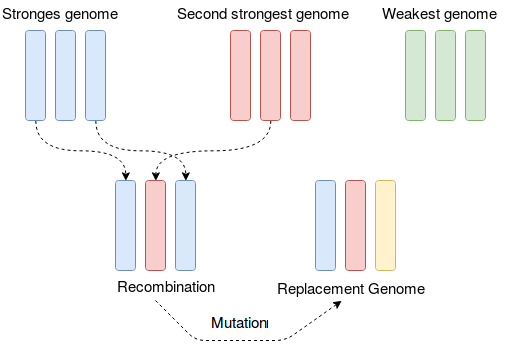
\includegraphics[width=0.8\textwidth]{Chapters/Experiments/search_algo/figures/Recombination_algorithm.png}
    \caption{Visualization of the recombination in algorithm 1c. In a three layer PathNet, the first and last layer in the recombination would be layer one and three in the winning genome, while layer two would stem from the second strongest genome. After a mutation of the recombination, the new genome replaces the loosing contender. Each color represents one genome from the tournament and yellow represents a mutation.}
    \label{fig:search.recombination_algorithm}
\end{figure}

Algorithm group two consists of two algorithms where the tournament size is changed between each task. This means algorithm 2a uses tournament size 2 for task 1a, task 1b uses tournament size 5 and so on until the last task of full cSVHN classification which uses tournament size 25. In algorithm 2b, this order of tournament sizes is reversed. It is expected that in visualization of metrics where a population average is calculated, such as training accuracy, an algorithm with high selection pressure will have abrupt value changes from one generation to the next. Low selection pressure would then give a more gradual change in such values. A change between these two curve types should be prominent or algorithms 2a and 2b.

Algorithms 3a and 3b have its selection pressure changed during each search for optimal paths. This means each algorithm behave the same for each task, which algorithms 2a and 2b did not. The change in selection pressure is gradual which means between tournament sizes 2 and 25, each tournament size is used about 4 times for a limit of 100 generations. It is obvious that an even distribution of tournament sizes on each generation is not possible when using a threshold accuracy as search termination, which is one reason searches in these experiments are limited by number of generations instead. 

\subsection{Metrics}\label{Search-experiment:Metrics}
Due to the experiment complexity and number of tunable hyperparameters there are a large number of search effects and attributes that could be investigated, so limitations have been introduced on which metrics are being addressed. 

As with the first-path experiments, module reuse between tasks will be an important metric. This number is highly effected by stochastic processes such as initialization of populations, mutation probability, layer sizes, path sizes and so on, but it is also the most intuitive and clear way to measure the transferability of modules. An assumption used behind this metric is that modules are able to contain some form of "memetic"\footnote{Memetic is used here to describe a quantification of knowledge in the same way "meme" is used by Richard Dawkins\cite{selfishGene} to describe a unit of cultural knowledge} unit knowledge. In this multi-task scenario, reuse can occur across multiple tasks, but focus will here be put on the total number of modules reused instead of separating the reuse across tasks. This is because if the effect on reuse between each search algorithm is small, the stochastic noise in reuse on between two tasks is not as descriptive of how an algorithm affects learning as with the total number. 

This reuse can indirectly be viewed by viewing the total number of modules used for all tasks. This total capacity use is both a result of the reuse of modules and the module size. Which means capacity could be used as a measure of how "effective" the learning under a search algorithm is. By using few modules in each task and reusing a high number of modules from previous tasks, little new parameter optimization have to be done. This effective parameter use would possible reduce the overall validation accuracy so in order to visualize the effectiveness of training, total number of training units applied to each module in each path would be a useful metric. 

To confirm the ordering of algorithms on the exploration/exploitation scale, a population diversity metric will be calculated\footnote{See \ref{Populationdiversity} for more details about computation} for each algorithm. The reduction in this diversity for each generation gives an indication of the convergence-rate of each algorithm. Those of high exploitation will quickly hone in on one genotype and optimize the weights along that path, while algorithms that focus on exploration will explore many more permutations of modules. 

During a search for an optimal path as solution to a given task, the total training effort spent on the task is spread across the modules available for training. This means when the search is terminated and the optimal path have been locked to future back propagation, most of the updated parameters are lost due to the re-initialization of PathNet. While total computational efficiency is not something addressed in this thesis, the ratio of used training effort to the total training spent on a task is an interesting metric. This ratio is highly dependent on how quickly a population converges to one optimal path. In scenarios where this occur fairly early on in the lifetime of the search, every subsequent generation performs training where almost all is along the optimal path. We would therefore expect algorithms with a high selection pressure to be placed high in a ranking of useful training. See \ref{Search-implementation} for description of a training unit. 

\section{Hypothesis}\label{Search-hypothesis}
The expectations for these experiments were heavily influenced by the results in the first-path experiments. When the training algorithms are viewed in a simplified context of only "exploration vs exploitation", we can place them on a scale between these extremes and discuss expected outcomes from each end of the spectrum. In this context, the Pick+Search learning scheme used in the first-path experiments would fall on the exploitation.

During a search, a given algorithm would have a population with consistently high diversity until the population converges to an optimal path. This convergence rate, and therefore also population diversity, is determined by which end of the exploration/exploitation spectrum we select our algorithm from. Since we limit ourselves by only changing the tournament size, we would expect a lower tournament size to lead to a low convergence rate and high diversity. This is a natural assumption to make considering the maximum change that occur in the population from one generation to the next. A tournament search with tournament size two has such a low selection pressure that from one generation to the next, only one instance of genotypic change is applied the the population\footnote{This is when the weakest genotype is replaced by the winner of the tournament}. The number of generations until the population have converged to one optimal path would therefore be higher under such a search, than a search where the selection pressure is considerable higher. 

A high selection pressure means strong phenotypes are favoured during the search. The algorithm would after one generation have a significant portion of its population genetically identical, ignoring possible genotypic traits caused by mutations. In the search context of finding an optimal path in a PathNet structure, evaluating a lot of similar paths to rank their fitness would lead to training the same modules multiple times. The next generation would then have a disproportionate fitness scores for some paths which would cause them to have a higher likelihood of winning the next generations tournament, and therefore quickly take control of a population by out performing all other paths. In such a scenario, the population have converged before other paths would have had time to adapt to pretrained modules interfaces, and the advantage PathNet brings with module transferability have been reduced, if not lost.  

For the locked tournament sizes the expectations are that high selection pressure causes high convergence and low module reuse between tasks. The low reuse would again cause more of the total number of modules in the PathNet to be locked after all tasks are learned. What the pressure would mean for validation accuracy is highly dependent on what tasks are learned, and from which domains they are selected. 
The opposite is true for the searches with a small tournament size. The low convergence leads each module to be trained in multiple permutation of PathNet subsets, and therefore also more transferable than modules trained during high selection pressure. If the searches are limited by the number of generations, and not by a threshold training accuracy, it would not be a surprise if the high tournament sizes yields paths with a higher validation accuracy for each task than those searches with low selection pressure. This is because each generation contain more effective training when there are more genotypes in the tournament. 
Not to be forgotten is the fact that all paths in one generation have the same final task specific layer.  Since this is shared across all paths, the high tournament sizes leads to orders of magnitude more training in the final layer for high selection pressures. For each generation, the final layer is trained once for each genotype being evaluated. Meaning after a hundred generations, it have been trained 2300 times more for a search with tournament size of 25 versus a tournament size of 2. 

% Variable tournament size between tasks: Dont know how it will affect
% Dynamic tournament size during search: Dont know

In addition to the static tournament sizes with a winner-replace-all crossover scheme, a search with recombination is tried together with tournament size three.  This should give a selection pressure even lower than that of tournament size two. From one generation to the next, there is still only one genotypic change in the population, but where the normal tournament search replace the loosing genotype with the winner, a recombination of the two strongest phenotypes replaces the weakest genome\footnote{With some additional mutation}.  Another way to view the step from tournament size two to size three with recombination is one with focus on the genome in the offspring that takes the weaker paths place in the population. Given the recombination scheme, it can be seen as a copy of the tournament winner, but with a strong mutation probability that is scaled down during the search. This down scaling comes from the convergence of the population. When the diversity is reduced, more and more paths will have a similar subset of PathNet. When selecting two paths with the same modules, the recombination will yield a path identical to both parents. So as a population grows closer to converging to an optimal path, it will consist of similar genomes and each recombination will give offspring closer to the population median than it would in a diverse population. 


In summary, a high tournament size is expected to shift the search algorithm in the direction of high exploitation which in turn should give a high performance on the different tasks. Low tournament sizes gives a high exploration of the different paths possible, which yields modules trained in multiple permutations of PathNet subsets. It is expected that this will lead to more module reuse, and generally have a lower capacity usage than algorithms of high selection pressure. 

It is hard to tell how the validated classification accuracy on the final task will be affected by the different algorithms. As with the previous experiments, the tasks selected might prove to be to simple which would hide much of the potential in transfer learning since a path of average since should be able to learn each task \textit{tabula rasa}.

% Some illustration of exploration vs exploitation: Hypothesis figure of where i think algorithms falls

\section{Implementation}\label{Search-implementation}
\subsection{PathNet}
The PathNet structure used for these experiments have three layers of 20 modules where each path may contain one, two or three modules in each layer. The 20 modules were selected to make sure there would be a a non-zero probability of selecting only empty modules for all tasks, even if all optimal tasks contained the maximum number of modules without any module overlap between tasks.

As with the refined first-path experiments, only convolutional modules with ReLU activation were used, but with two channels each instead of the one in first-path. To verify, a random path with these hyper-parameters were created and applied to the task of full cSVHN classification and was able to reach a satisfactory performance within a reasonable training time. The Adam optimizer were used during back propagation with a learning rate of 0.0001. 

Each convolutional module also includes a batch-normalization operation and the last module ends in a max-pooling before the output is flattened and passed through the final unique classification layer. 

As there is a resolution difference between the cSVHN set and MNIST, an additional preprocessing step were applied to the MNIST set. A 2 pixel border of zeros were added to change the dimensions from 28x28 to 32x32. cSVHN images has three-channels of RGB values so the single channel of padded MNIST images were repeated in every color-channel to reach the final dimensions of 32x32x3.  

\begin{figure}[h]
    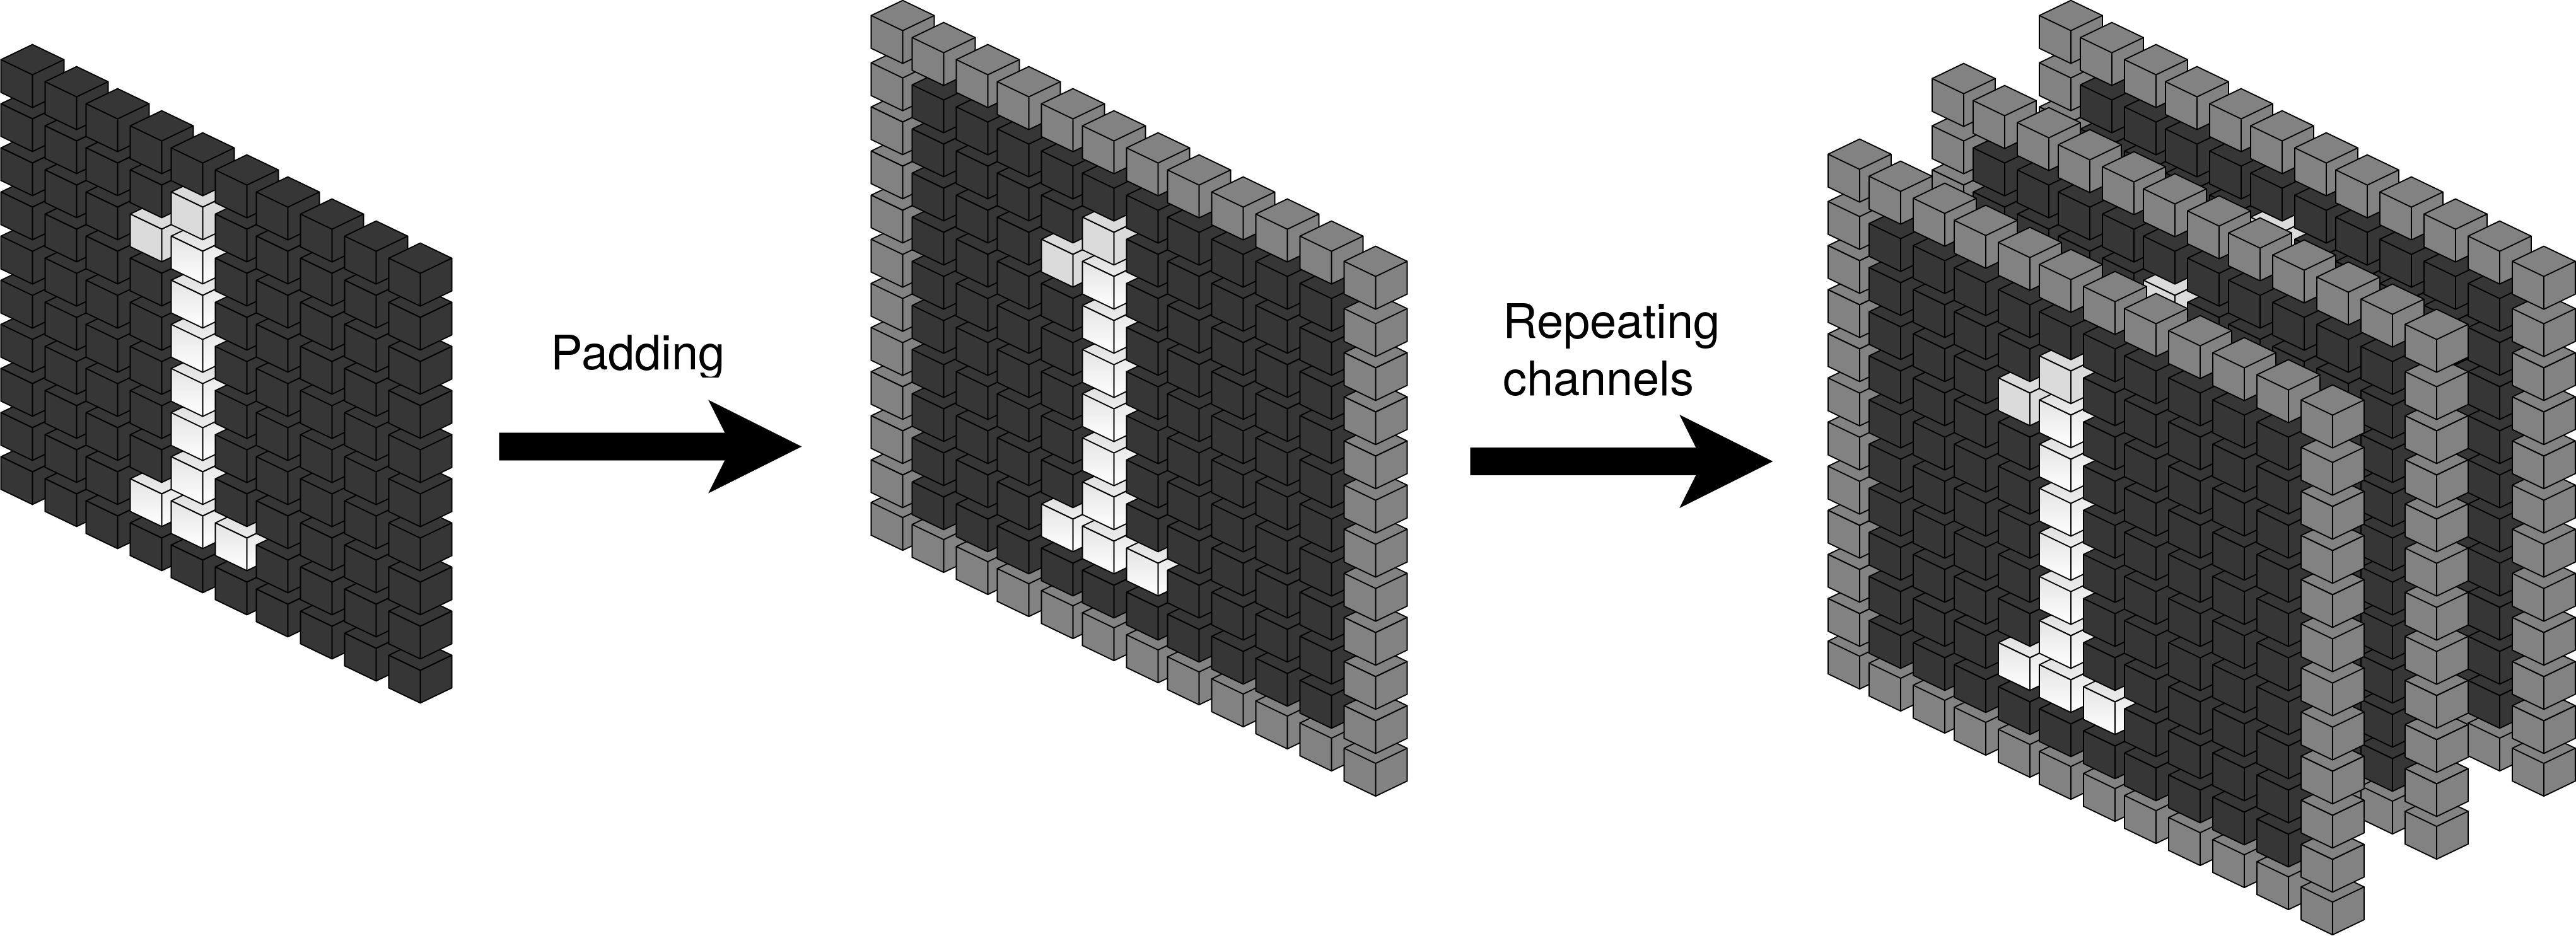
\includegraphics[width=\textwidth]{Chapters/Experiments/search_algo/figures/MNISTpadding+repeating.png}
    \caption{How MNIST is adapted to have same dimensions as cSVHN. Illustration use dimensions 12x12x3 while cSVHN and adapted MNIST use 32x32x3}
    \label{fig:MNISTpadding}
\end{figure}

\subsection{Tournament Search}
The tournament search uses a population size of 64, and as discussed, a winner-replaces-all replacement scheme between generations. Instead of using a accuracy threshold as in the previous experiments, the search terminates after 100 generations. A important feature of PathNet is the way learning is done. Since network back propagation occur during path fitness evaluation, the locked number of generations limit the amount of training that is allowed. In the original paper, fitness is set as the negative training error which is reached for each path after it have been trained for one training unit of 50 mini batches of size 16. This is an reasonable way of evaluating the fitness of a path when using a small tournament size, but as the tournament size have been increased tenfold for the algorithms with high selection pressure, fitness is calculated differently in these experiment. 

The problem of directly using the training error as fitness is that the error changes whenever weights along a path is updated. An extreme example can be used to present the underlying problem with this. 

Take a tournament selection of 25 genomes containing 24 identical paths and one different path with some module overlap to the others and which is evaluated first. One scenario could be that the first unique path is evaluated to a high fitness, when the next path evaluated, the weights in the modules which overlap between the two are updated. The evaluated fitness of the first path is now outdated, and for every subsequent path, this fitness might get worse and worse if the parameters in the overlapping modules move to an area of high error in the context of the first paths other modules. After all fitness evaluations, the first path now stands with a high fitness, which might be larger than that of all other paths in the tournament. Then all other paths in the tournament is replaced with the winning path even if its actual fitness might have become significantly reduced during the evaluation step. Due to this, the fitness of paths in a tournament is calculated in a separate step for these experiments. After a subset of the population is selected for a tournament, all paths in that tournament are trained for one training unit. When training is completed, each path is evaluated by using a new subset of the training data for validation. This way, the order in which paths are validated does not affect the fitness score, which is the classification accuracy reached during the validation step. 
The order of paths still affect the the training but the fitness used for selecting a tournament winner is the "true"\footnote{Fitness is still calculated on the basis of the training data-set, which means it might become overly optimistic over time. Over-fitting during training is discussed in the context of another experiment} fitness score.

The same reason influence the final step of the tournament search. When the limit of a hundred generations is reached, all paths in the population is evaluated again. Since the true fitness of a path might change from one generation to the next, only the paths participating in the final tournament has its true fitness score as part of the selection of the optimal path. As with the evaluation step, the final fitness of a path is the reached classification accuracy of one training unit (50 mini-batches of 16 samples). Using an actual validation set for this step might yield better, or at least more accurate, fitnesses to use as a basis for path-selection, but that would significantly increase the run-time of an already time intensive experiment. 

\section{Results}\label{Search-results}
Due to the experimentation being time-consuming, each algorithm were run 10 times and logs were saved after each experimental run of each algorithm. The following plots have been separated in three groups based on subject: paths, search and training. 

\subsection{Paths}
\begin{figure}[p!]%[h]
    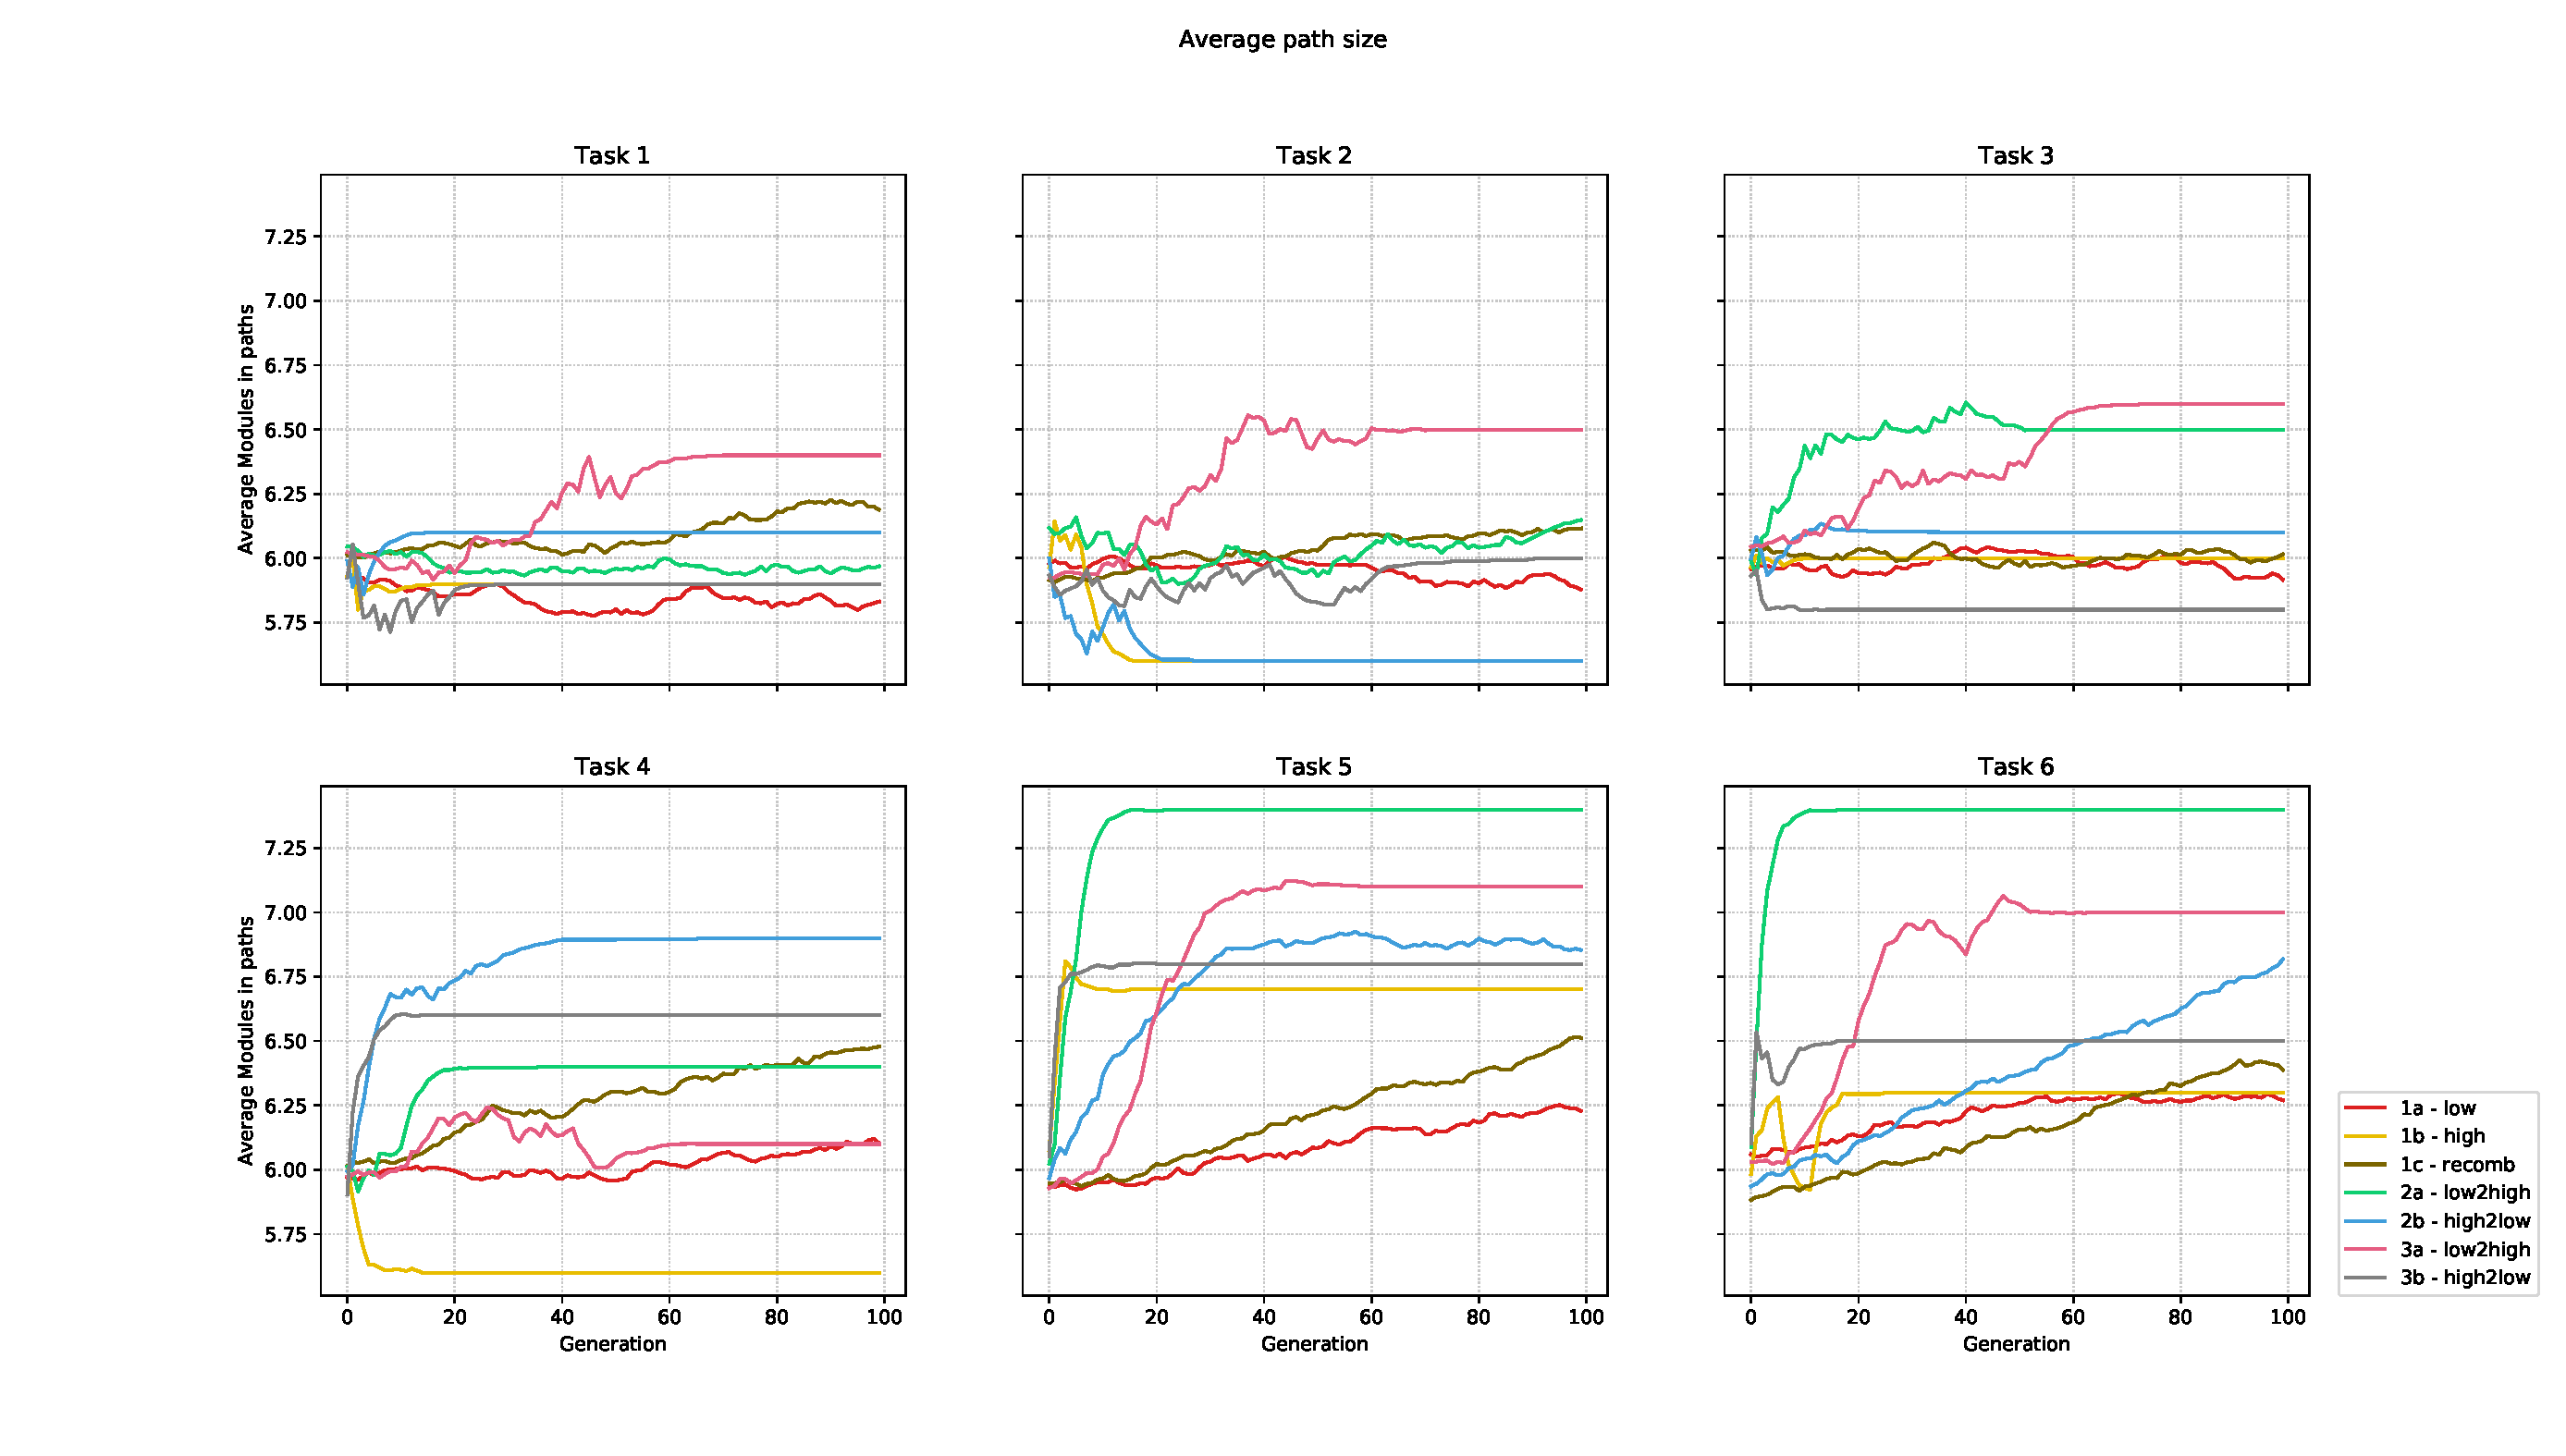
\includegraphics[width=\textwidth]{Chapters/Experiments/search_algo/figures/Average_path_size.pdf}
    \caption{Change in average path size for each tournament scheme plotted for each task.}
    \label{fig:search.avg_path_size}
\end{figure}

Figure \ref{fig:search.avg_path_size} visualize the average path size within the average population for all generations. Each subplot is for one Task and the search for that tasks optimal path. As each path contains between three and nine modules, the average path size is six and this is reflected in the plots where this is the initial value for the first generations. Each search starts with a randomly initialized population of paths. Note the span of sizes plotted reach from around 5.5 to around 7.5, which indicates the average initialized size of 6 does not contain enough capacity as more often than not, the searches converges towards larger path sizes, especially for the later three tasks based on the cSVHN set. 

A feature of this plot is the steep jump and quick convergence to a size for the searches with high selection pressure in for the early generations. Since mutation only causes the index of a module to change by a value between -2 and 2, the size of a path can not change during mutation \footnote{A path can not include the same module multiple times. If a module is mutated to overlap an existing one, it is removed. This causes the path to contain fewer modules, so mutated modules are added back in until original path size is reached.}. This means when algorithms with high selection pressure converges to a size early in the search, the size of paths can never change. For searches with low selection pressure (algorithm 1a, 1b, 2a for the earlier tasks and 2b for the later tasks), the generation limit of 100 is to low to let them reach an optimal size. 

\begin{figure}[p!]%[h]
    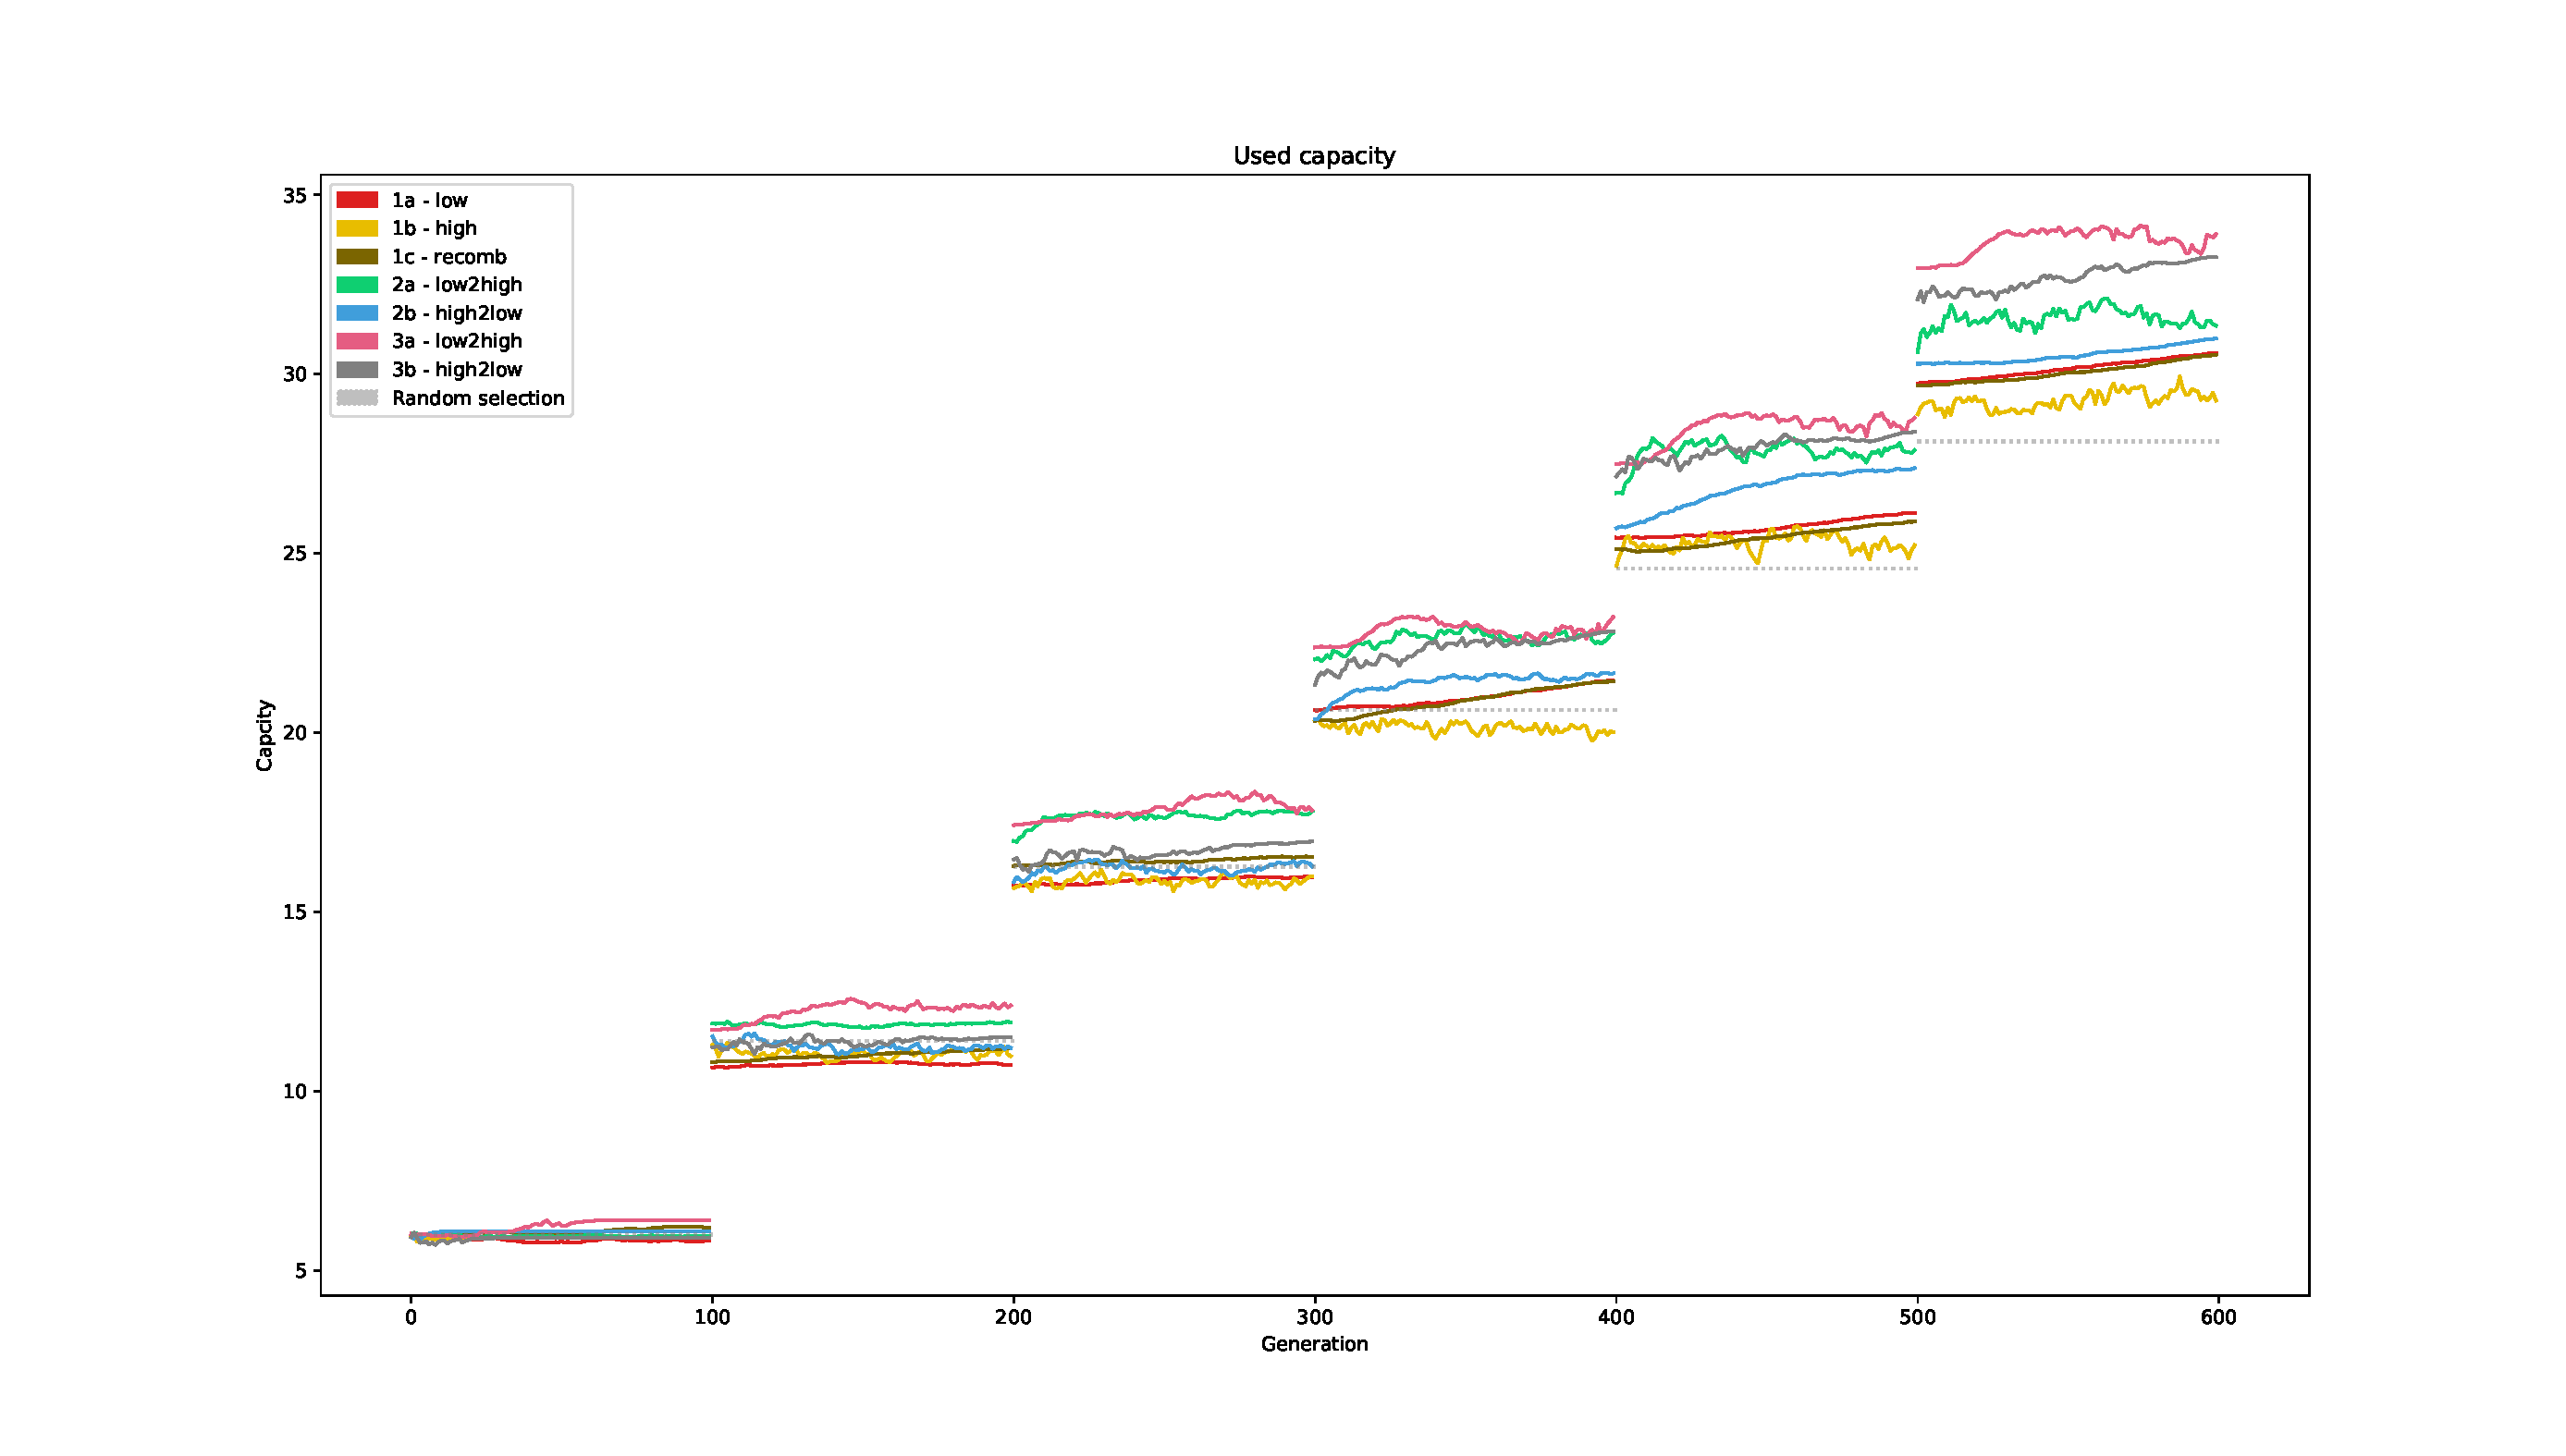
\includegraphics[width=\textwidth]{Chapters/Experiments/search_algo/figures/Capacity_pr_generation.pdf}
    \caption{The average number of used modules during the multi-task learning sequence. Each jump is caused by the saving of an optimal path and then starting a new search for a new task. }
    \label{fig:search.capacity}
\end{figure}

In figure \ref{fig:search.capacity} we can see some of the influence of path size in the average cumulative amount of capacity used during all generations. As with plot \ref{fig:search.avg_path_size}, the curves starts at capacity 6 and for the same reason. 

For task 4 the capacity usage have separated for the three algorithm groups. All algorithms with static tournament size use less modules in the total PathNet than the other algorithms, and algorithms with changing tournament size between tasks use less than group three. Note that all algorithms has a higher capacity usage than the dotted gray line which marks the amount of module reuse that would have been reached for 6 tasks if all paths had a random module selection\footnote{These values are reached by a Monte Carlo approach where \(10^{6}\) sequences of 6 random paths were selected in the same sized PathNet and the capacity used averaged.}.

\begin{figure}[p!]%[h]
    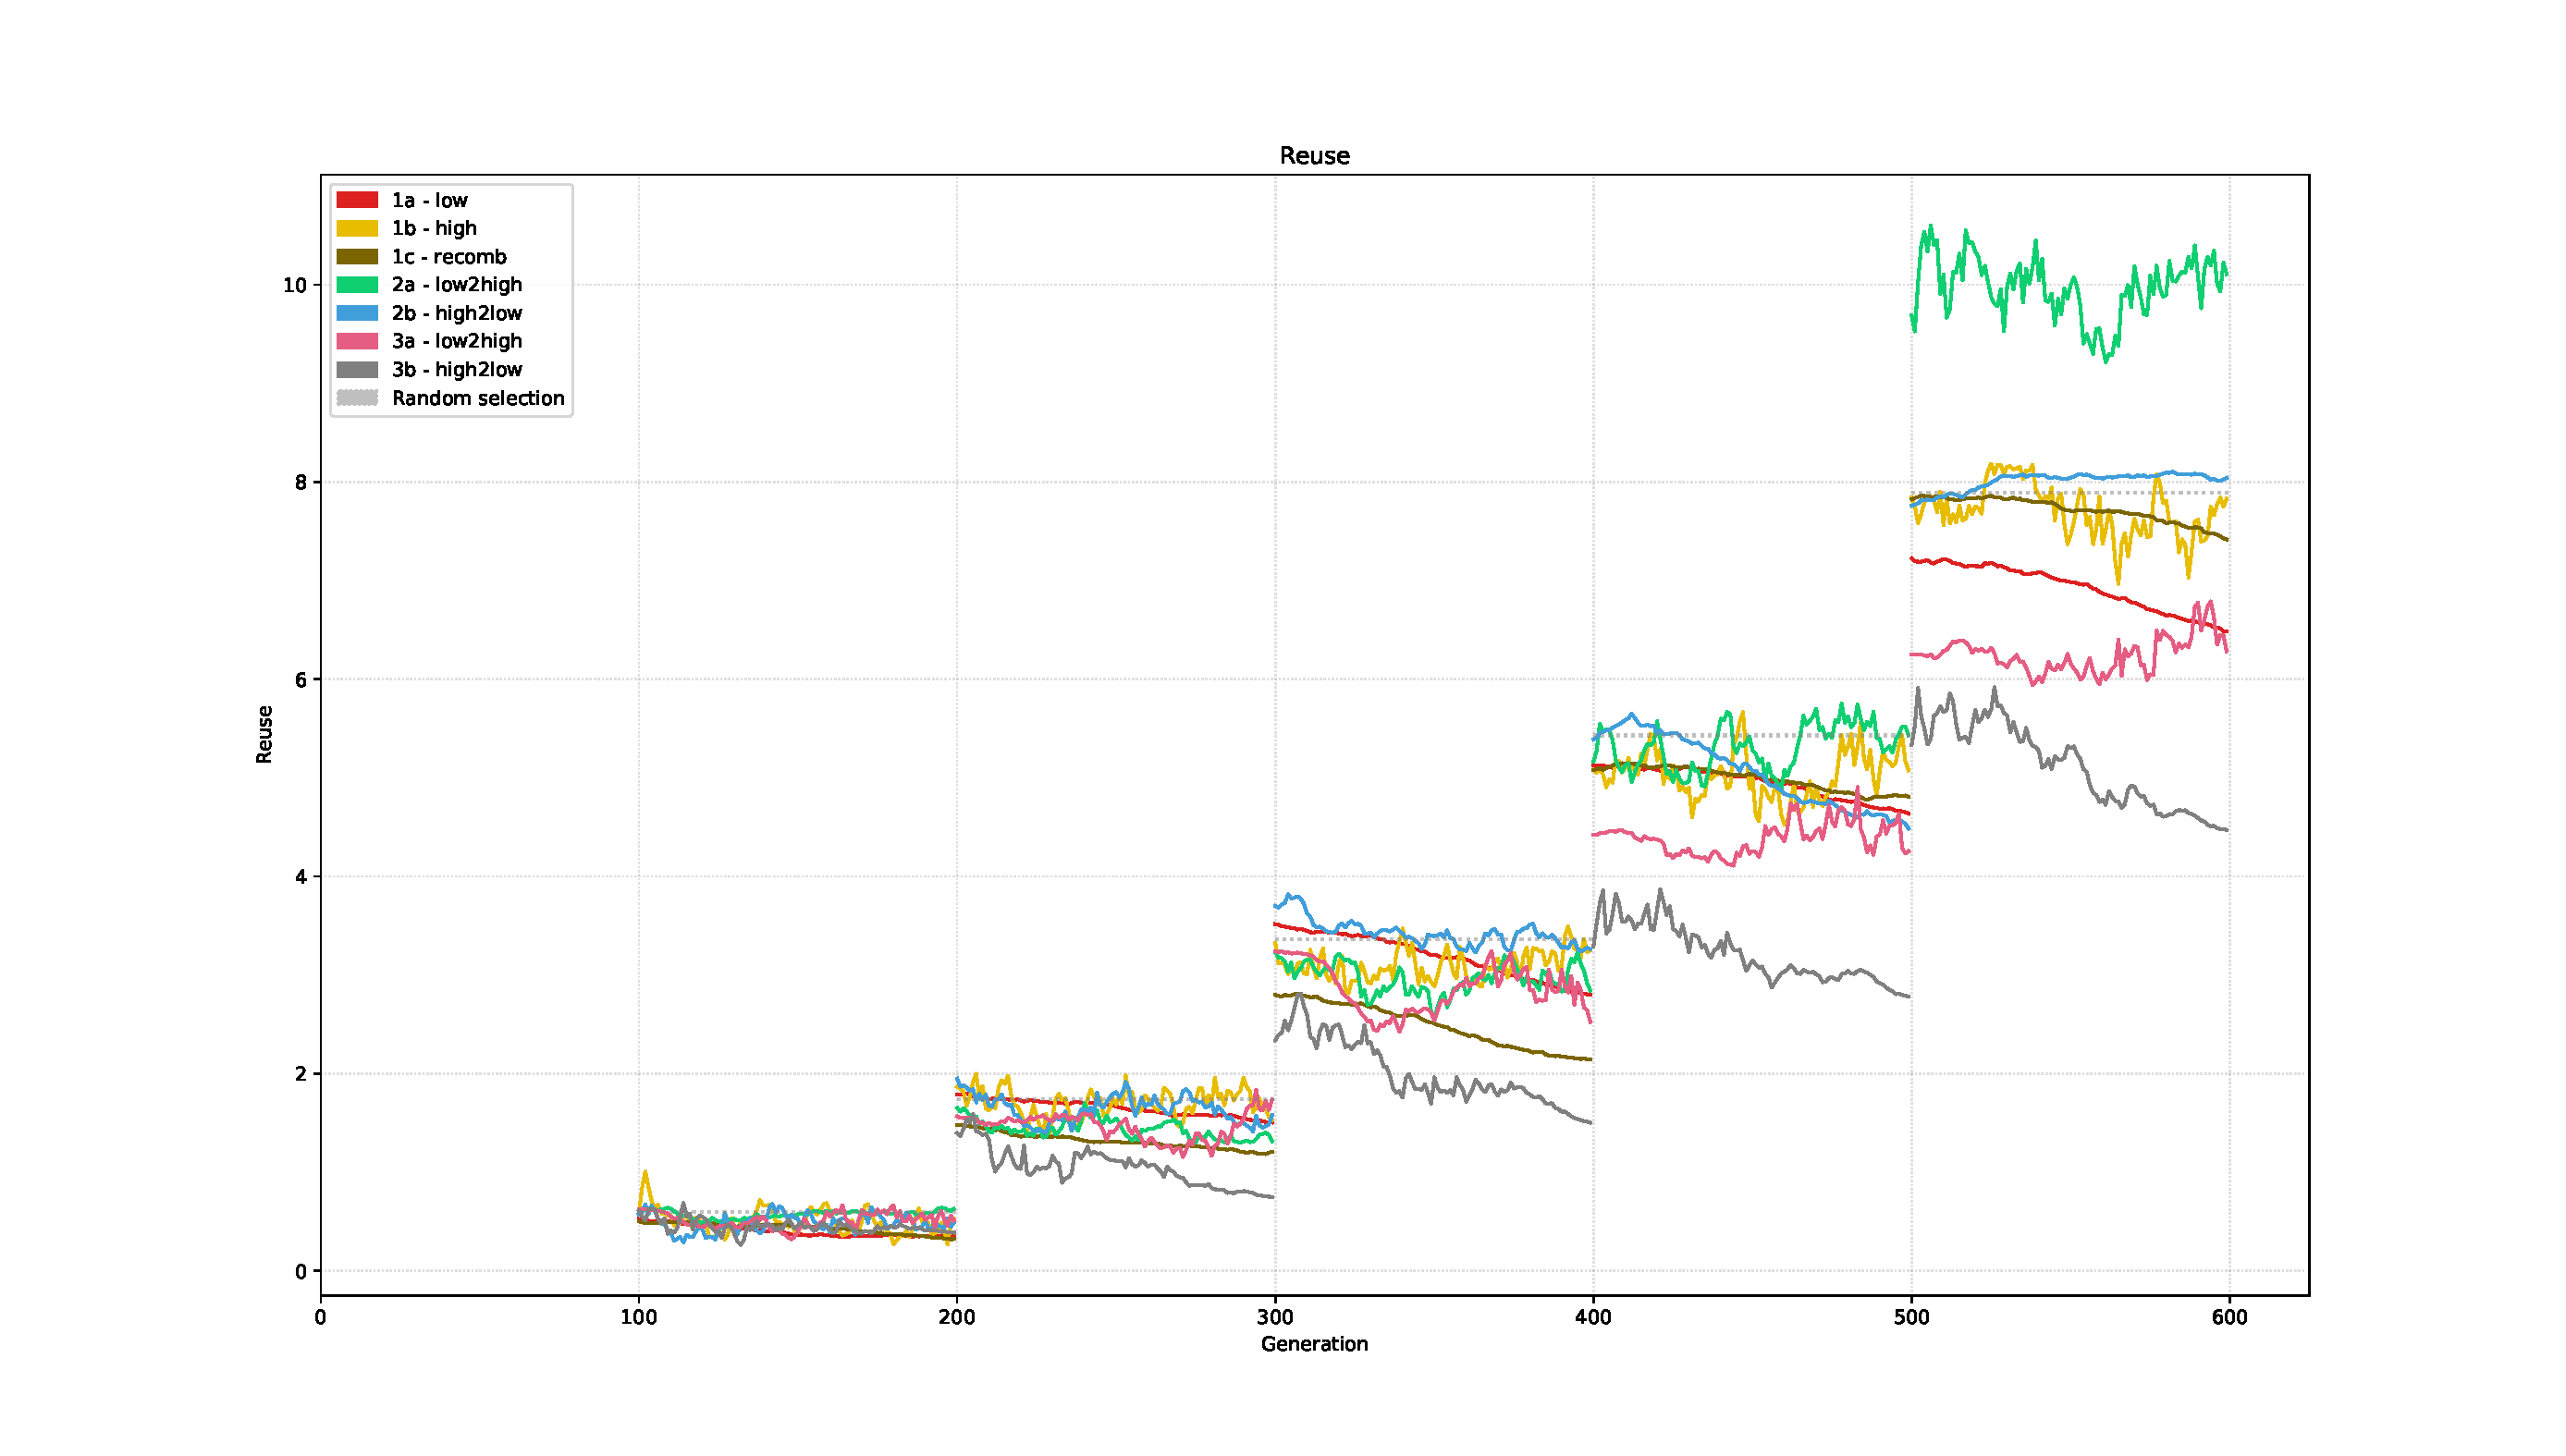
\includegraphics[width=\textwidth]{Chapters/Experiments/search_algo/figures/Module_reuse_pr_generation.pdf}
    \caption{The average module reuse during the multi-task learning sequence. Each jump is caused by the saving of an optimal path, and the next task having more locked modules to reuse. The first 100 generations does not have any previously learned knowledge to reuse.}
    \label{fig:search.reuse}
\end{figure}

The similar plot \ref{fig:search.reuse} show how the average amount of module reuse change during the generations. As with plot \ref{fig:search.capacity}, the dotted grey line represents the amount of module reuse in a random selection of modules\footnote{These values are reached by a Monte Carlo approach similar to plot \ref{fig:search.capacity}.} instead of search. Between the two last tasks we see a large jump in module reuse for algorithm 2a compared to the rest. The dynamic tournament size algorithms 3a and 3b has the least reuse for task 4 and 3b seem to lower its reuse significantly during each search. 

When visualizing search features for the different algorithms that stem from different generations during each search, the algorithms using a high tournament size have curves undergoing rapid changes and algorithms using low tournament sizes have curves with more gradual changes. Plot \ref{fig:search.reuse} is no different, which can make it hard to tell if there is an increase or decrease in reuse for algorithms 1b and 2a for the last 600 generations. 

\subsection{Population Diversity}
\ref{fig:search.hamming_diversity} visualizes the average calculated population diversity for each algorithm for each task. As this metric is dependent on the size of population as well as the number of genes in a genotype, the value at one point in the generation is not depictive of anything, but instead, the overall trend of the measure indicates at what rate the algorithm converges. 

\begin{figure}[p!]%[h]
    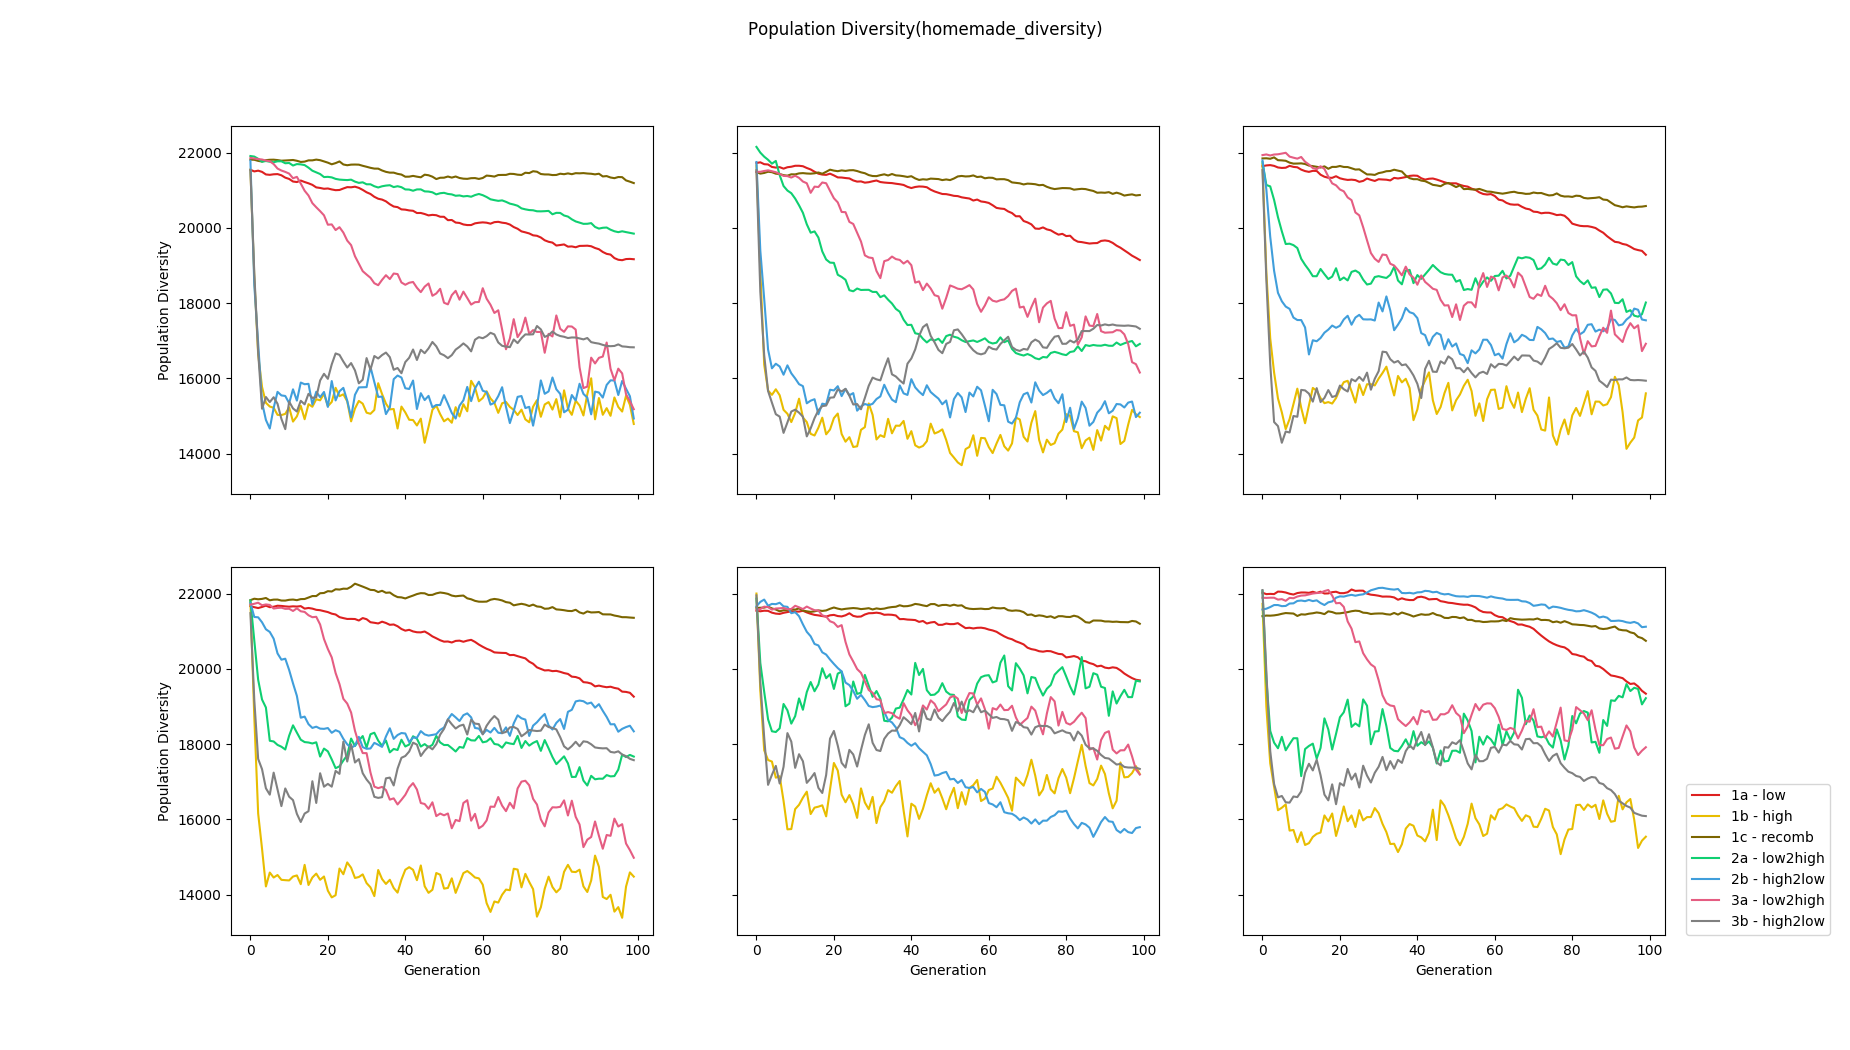
\includegraphics[width=\textwidth]{Chapters/Experiments/search_algo/figures/Average_population_diversity_reduced_hamming.png}
    \caption{The average pairwise Hamming distance within each generation is used as a measure for population diversity. Each subplot (in order left to right) is each task in trained order.}
    \label{fig:search.hamming_diversity}
\end{figure}

As with plot \ref{fig:search.avg_path_size}, high selection pressures lead to rapid changes in diversity. This is because the searches with high selection pressure have a high tournament size compared with the population size. When a generation is over and  the tournament winner replace all losers, the population makes a large shift in diversity unless most of the tournament participants have a similar genome. At that point, the probability that the population have converged is quite large. 

\begin{figure}[p!]%[h]
    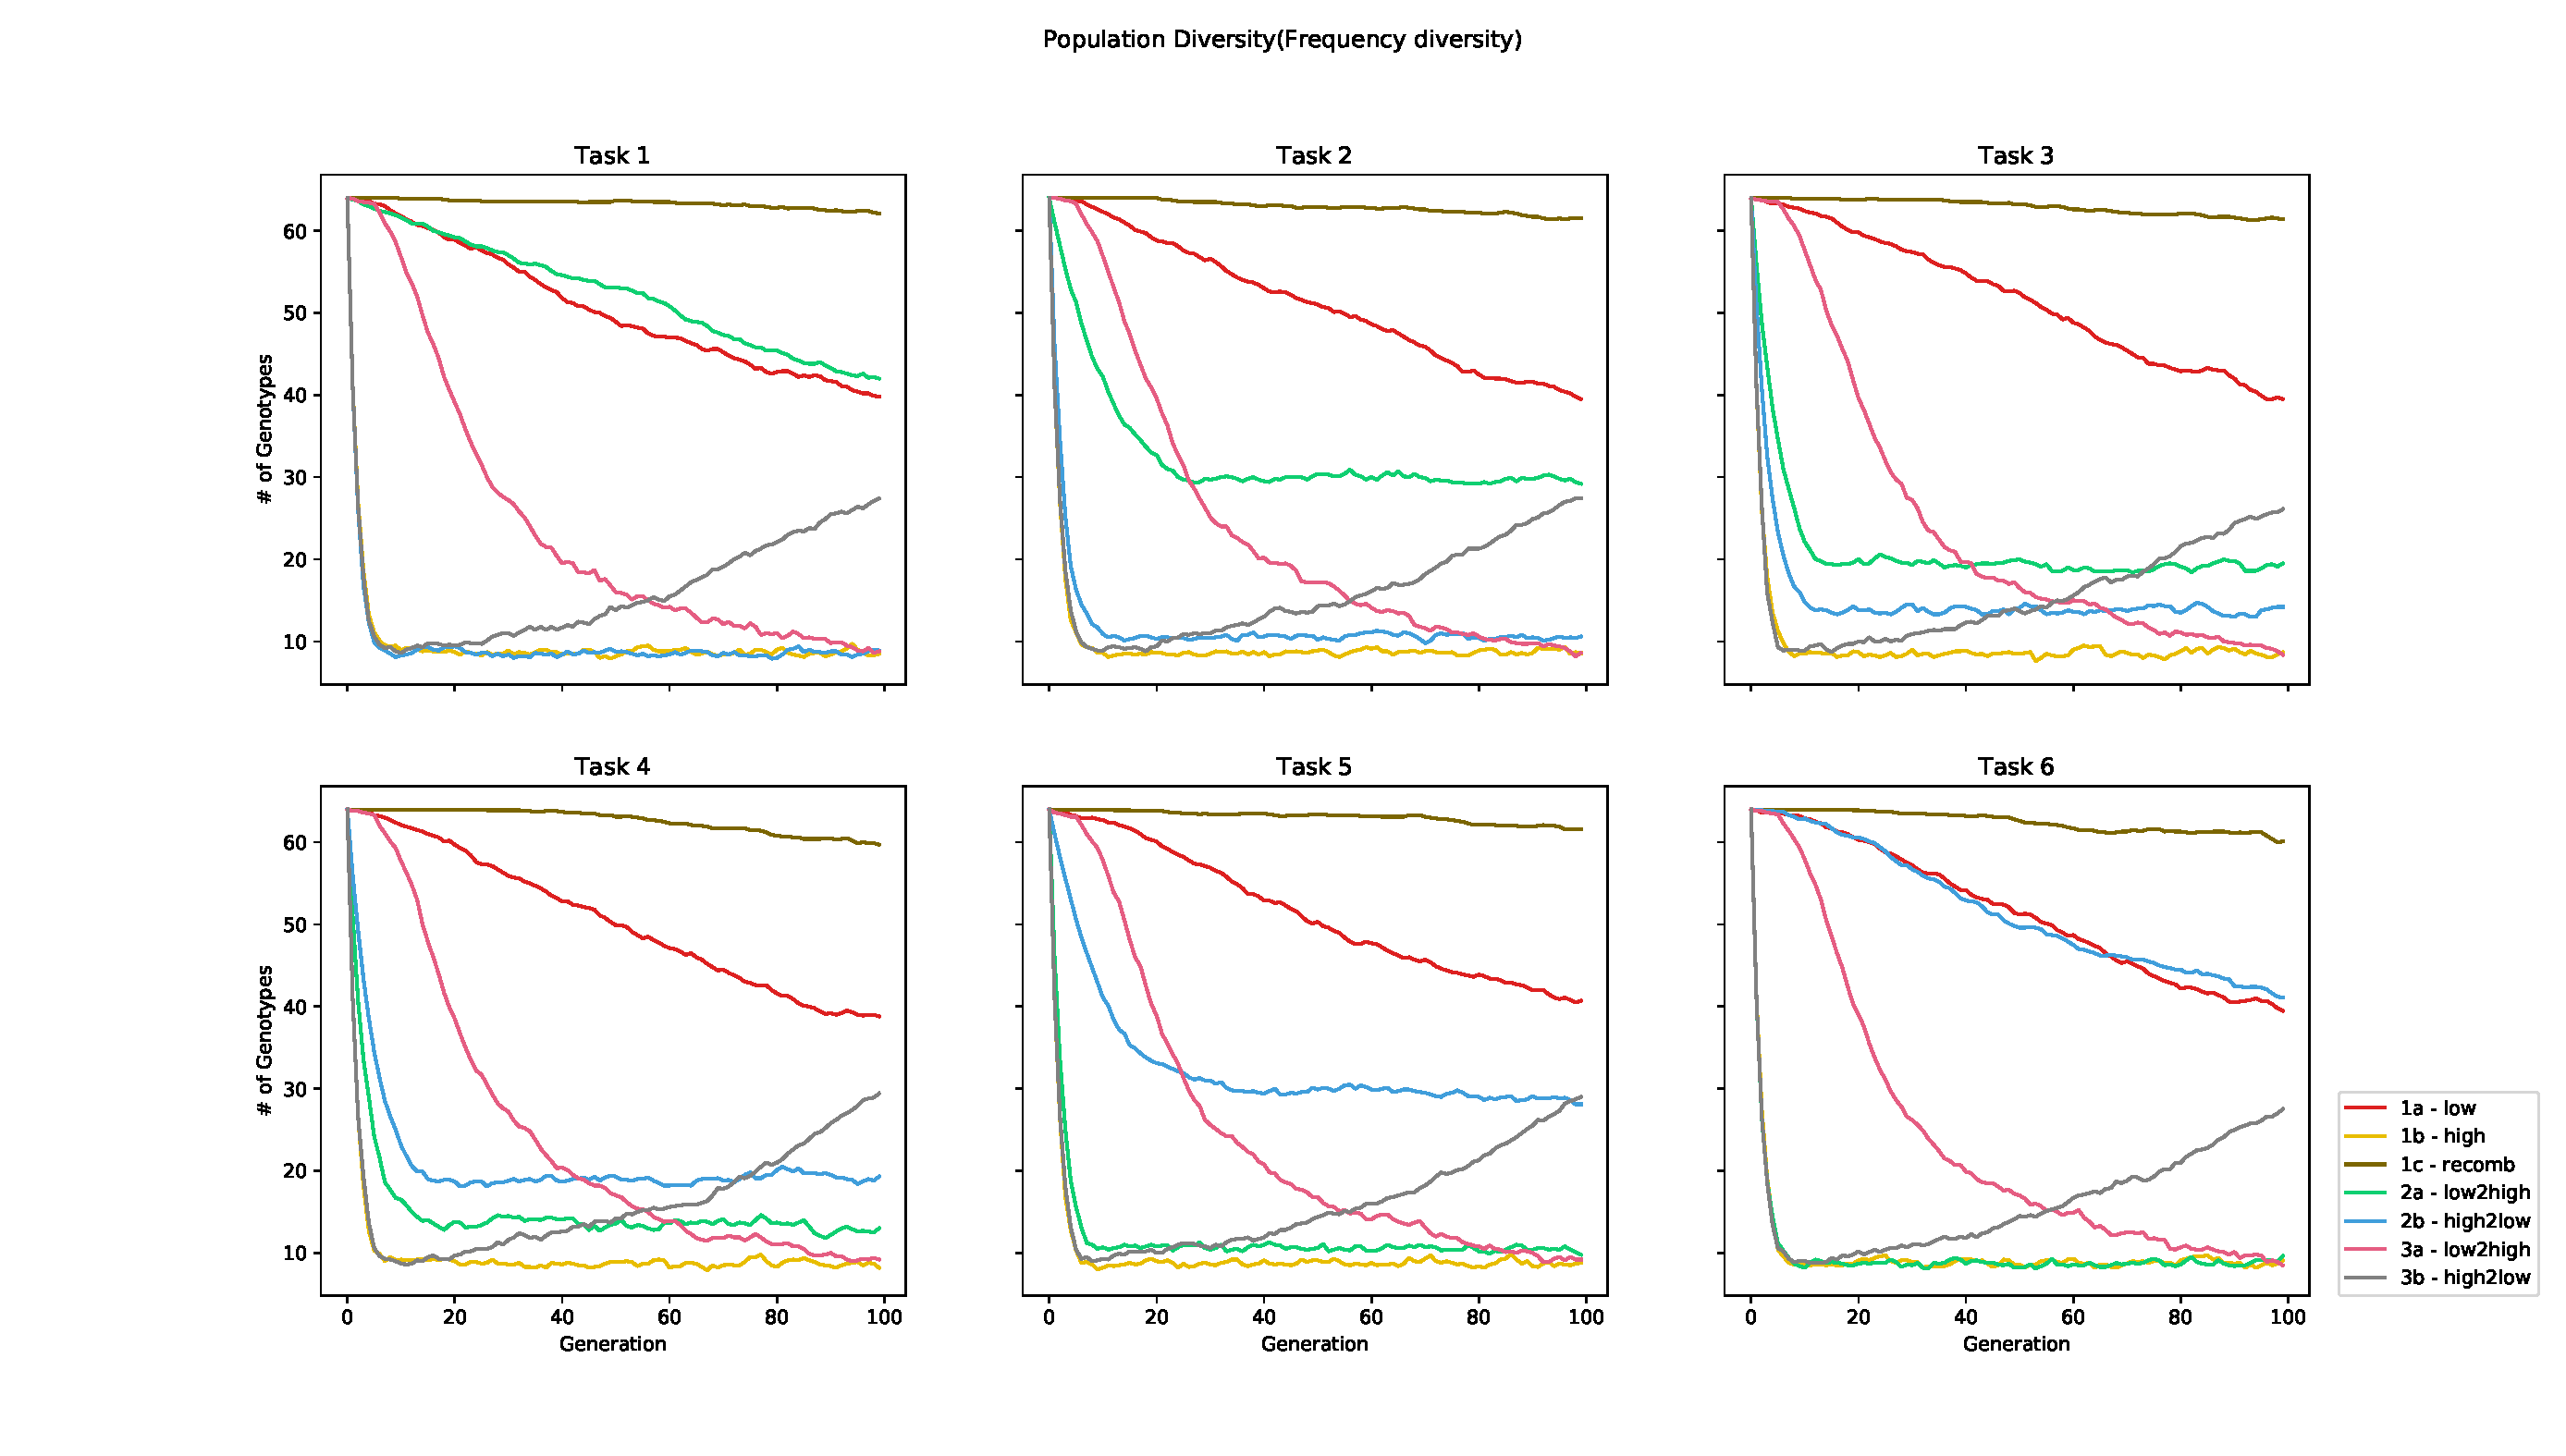
\includegraphics[width=\textwidth]{Chapters/Experiments/search_algo/figures/frequency_diversity_unique_path_count.pdf}
    \caption{The number of unique paths within a population. Plotted for every task and every algorithm.}
    \label{fig:search.frequency_diversity_unique}
\end{figure}

The Hamming distance between two binary genomes gives what is essentially the edit distance and not a measure of the fundamental difference between the genomes. This means the Hamming metric is accurate and quite descriptive when looking at one gene at a time, but for larger genomes can be somewhat misleading in some circumstances. Take for instance, a population consisting of three even groups of three types of genomes. If one group is replaced with genomes from the two other groups such that the population consists of two equal parts of each genome, the diversity of the whole population have gone down\footnote{This is fairly obvious since we in this scenario is left with only two types of genomes, while we started with three}, but the pair-wise Hamming distance might have gone up. Because of this, it is hard to tell if the constantly high diversity levels is caused by using pair-wise Hamming distance as metric, or for instance high mutation probabilities. This effect becomes clear when comparing plot \ref{fig:search.hamming_diversity} with plot \ref{fig:search.frequency_diversity_unique}. This plot visualizes the amount of unique paths in a population and has therefore some problems as a diversity metric that Hamming distance does not. A mutated genome would be considered to be a similar genotype to its original state, and a pair-wise Hamming distance would reflect this by only counting the small genome change between these two. On the other hand, a unique genotype frequency metric would count these two genotypes as completely different.

\subsection{Training}
\begin{figure}[p!]%[h]
    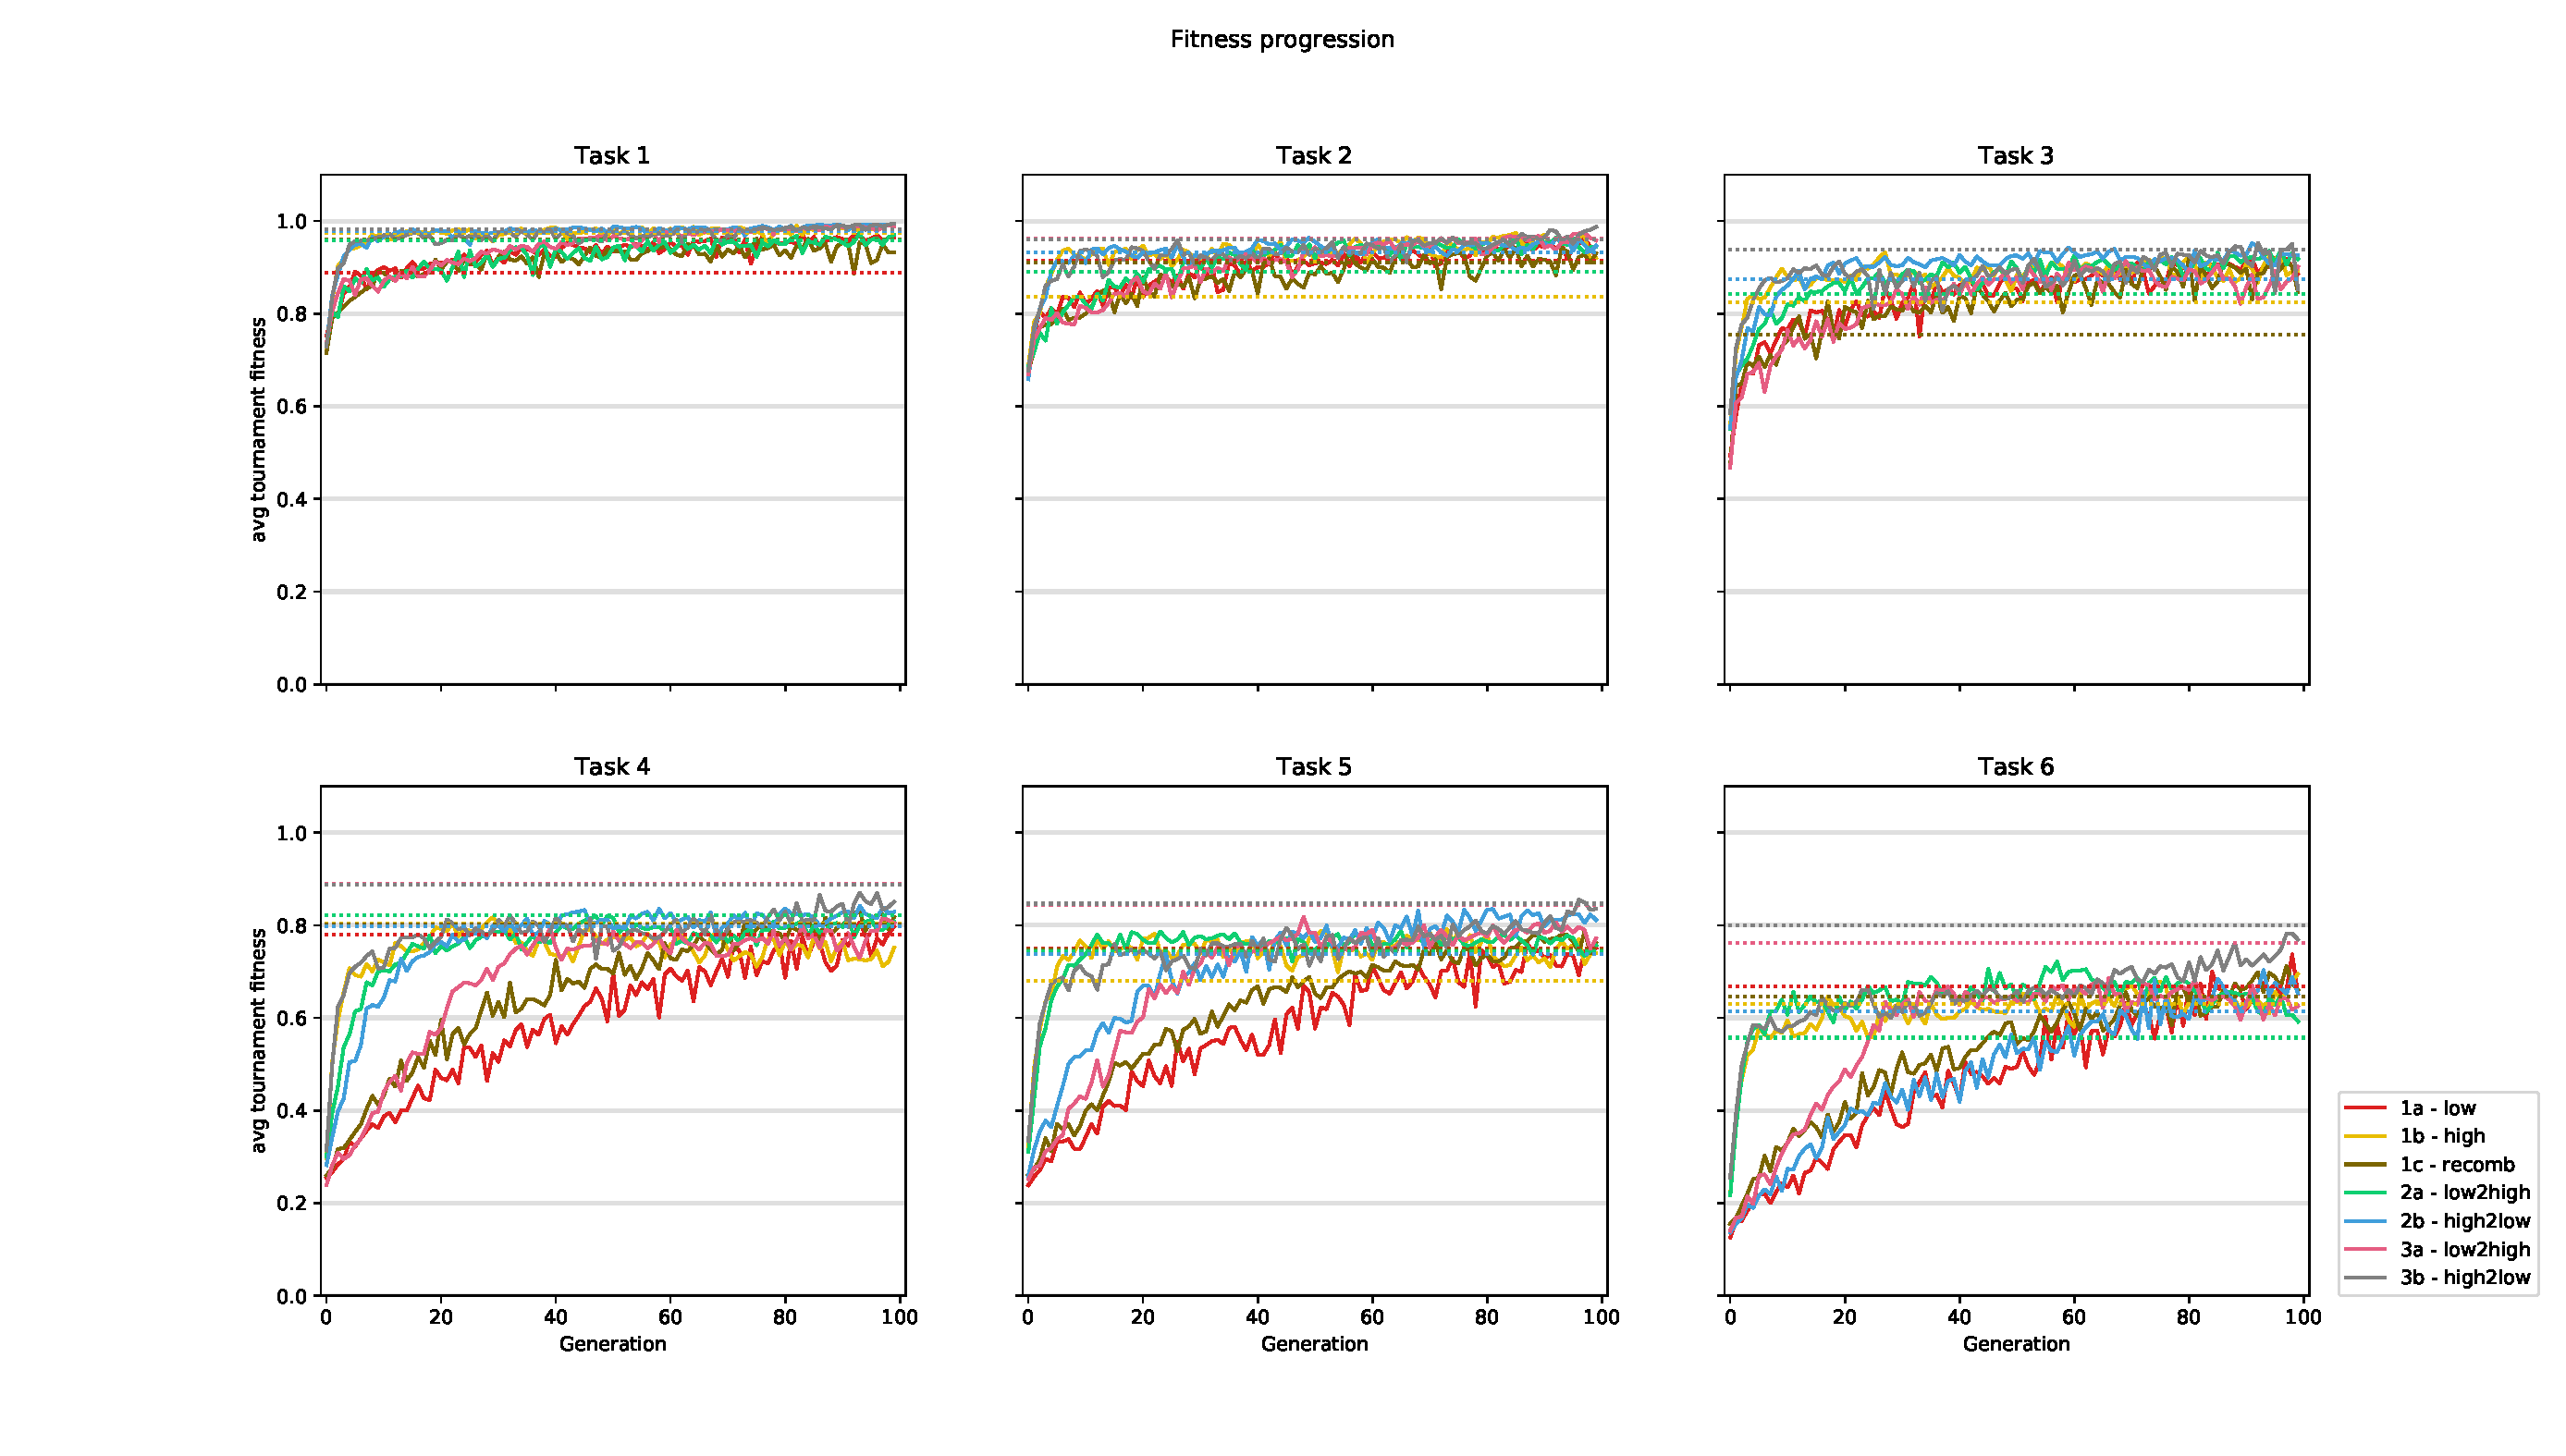
\includegraphics[width=\textwidth]{Chapters/Experiments/search_algo/figures/Training_accuracy.pdf}
    \caption{Average training accuracy during search. The dotted lines is the average achieved validation accuracy for that task and that algorithm.}
    \label{fig:search.accuracy}
\end{figure}
As the training of each path is done during and controlled by the search, how the average training accuracy develops gives an indication of how quickly the algorithms are able to influence the overall PathNet to learn a task. As discussed previously, the act of training one tournament of genomes effect the previously evaluated fitness values. Because of this, the populations average fitness values would be a highly misleading metric to use and therefore what is plotted here is the average fitness score achieved within a each generations tournament. Also plotted is the average validation accuracy reach for each algorithm. This validation score is only calculated after an optimal path have been found for each task, and can therefore not be viewed as a function of generation number. 

\begin{figure}[p!]%[h]
    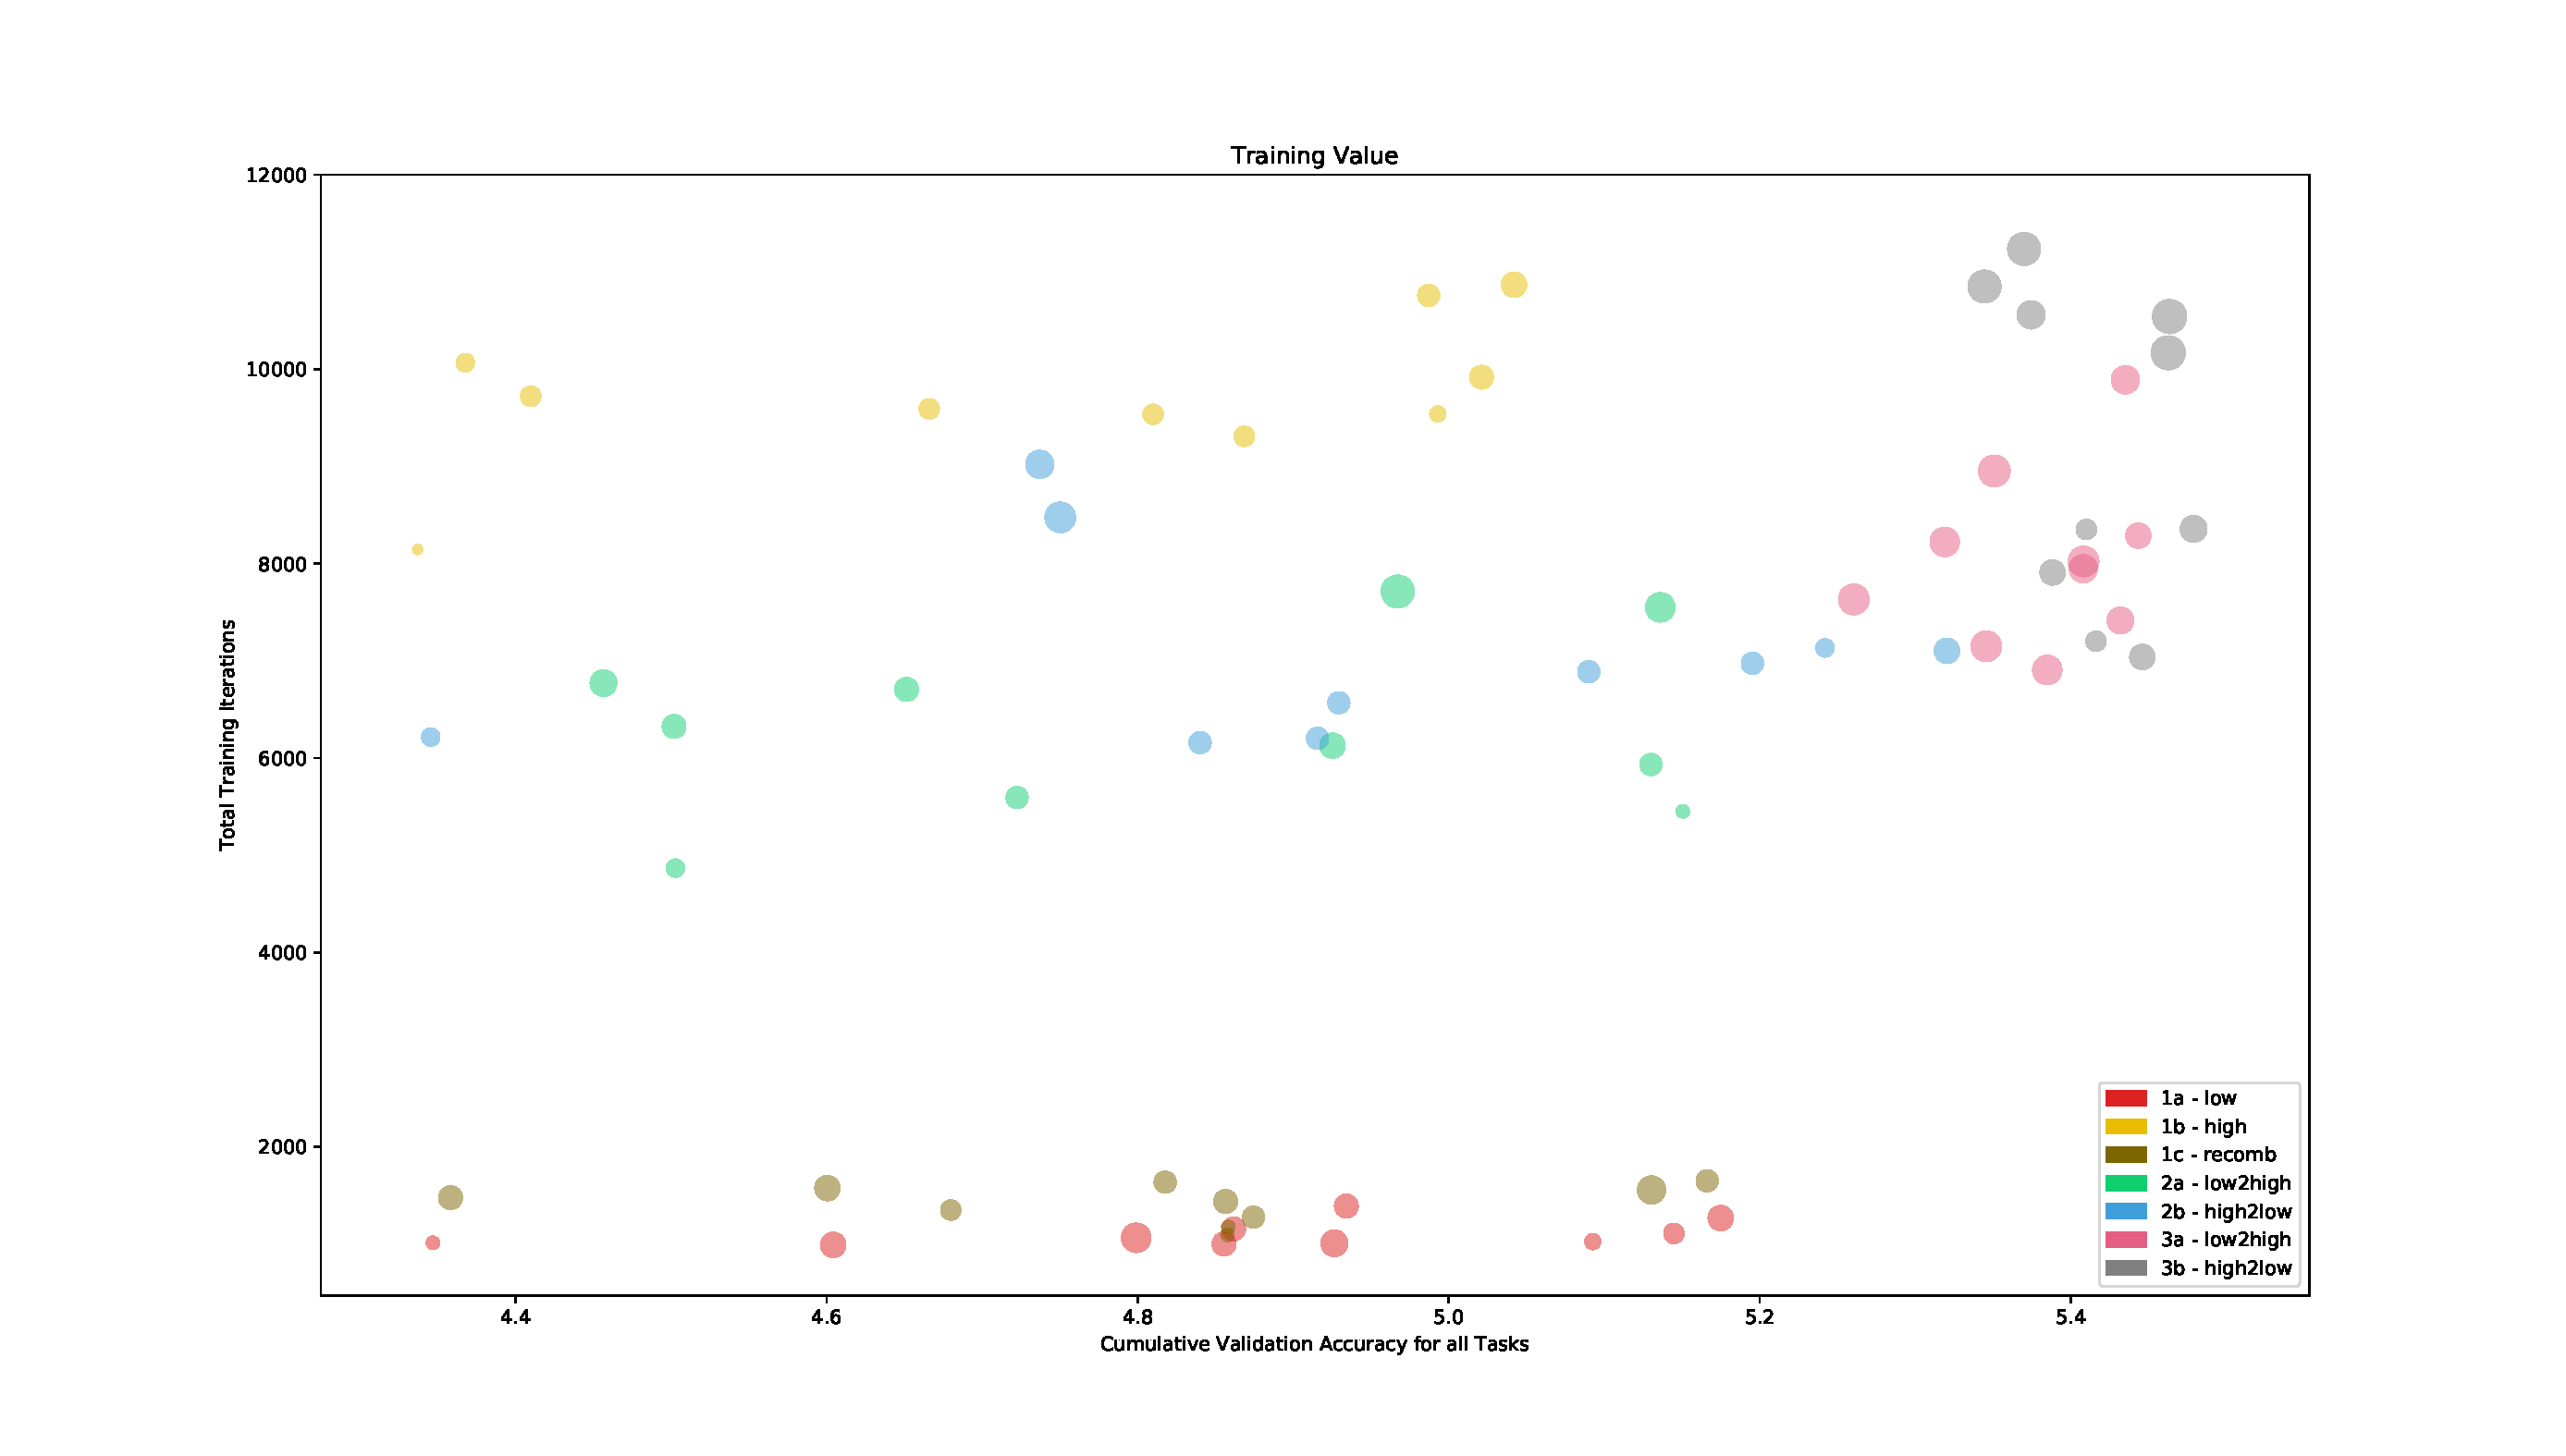
\includegraphics[width=\textwidth]{Chapters/Experiments/search_algo/figures/Training_value.pdf}
    \caption{The total amount of training in all optimal paths for each multi-task learning sequence plotted against the cumulative validation accuracy reached for that sequence. The circle size corresponds to the total number of used PathNet modules.}
    \label{fig:search.training_value}
\end{figure}

The training value plot \ref{fig:search.training_value} the amount of training each multi task sequence went through for all 6 tasks. As expected, algorithms with high tournament size (algorithm 1b) have the higher amount of training units, while the low tournament size algorithms (algorithm 1a and 1c) undergo the least training.

The x axis in this plot is the cumulative validation accuracy for all tasks within the multi task sequences, meaning algorithms that cluster on the right side of the plot have a better accuracy over all. 

Lastly, the circle size reflect how much total capacity was used in the PathNet for each experimental run. Described simply, small circles in the bottom right corner means the algorithm used few weights, took little training and had a good classification accuracy. Comparatively, large circles in the top left corner used a relatively large amount of weights, took long to train and had a low return on investment in classification accuracy. The clear clustering of experimental runs for each algorithm spatially is expected in this plot as the number of training units is easy to predict from the tournament size, however, the clear divide between algorithm 2a and 2b is surprising.

\section{Discussion}
\textbf{EDIT NOTE: Rerun of experiments might change results}

Unraveling the amount of information that came as a result of these experimental runs can lean towards the disorienting if not chaotic. In an attempt to be able to discuss the plots mentioned in the previous section, the algorithms are juxtaposed within selection pressure groups first before comparisons are made between them. 

\subsection{Low selection pressure}
Algorithms 1a and 1c have the lowest convergence rate, and as a result of this have also the most gradual changes during each search. Given the modules under these algorithms experience the least amount of training we would expect these to reach a lower classification accuracy, but performing a one-way ANOVA test of the null hypothesis
\begin{equation*}
    \label{eq:H0.accuracy.notLowPressure}
    H_{0}:\bar{\mu}_{1_{a}}=\bar{\mu}_{1_{b}}=\bar{\mu}_{1_{c}}=\bar{\mu}_{2_{a}}=\bar{\mu}_{2_{b}}
\end{equation*}
where \(\mu_{x}\) is the mean validation accuracy of algorithm x, gave no p values under the significance level of 0.05\footnote{Significance level 0.05 is used throughout this thesis.}, and the alternate hypothesis
\begin{equation*}
    \label{eq:H0.accuracy.notLowPressure}
    H_{A}:\bar{\mu}_{a_{i}} \neq \bar{\mu}_{a_{j}} 
\end{equation*}
is true for at least one pair of algorithms \(a_{i}\) and \(a_{j}\), where both \(a_{i} \land a_{j} \in A\), and where \(A\) is the set of all algorithms. Looking at figure \ref{fig:search.validation}, the reason for the lowered mean in plot \ref{fig:search.accuracy} seems to be caused by an outlier in the data.

\begin{figure}[p!]%[h]
    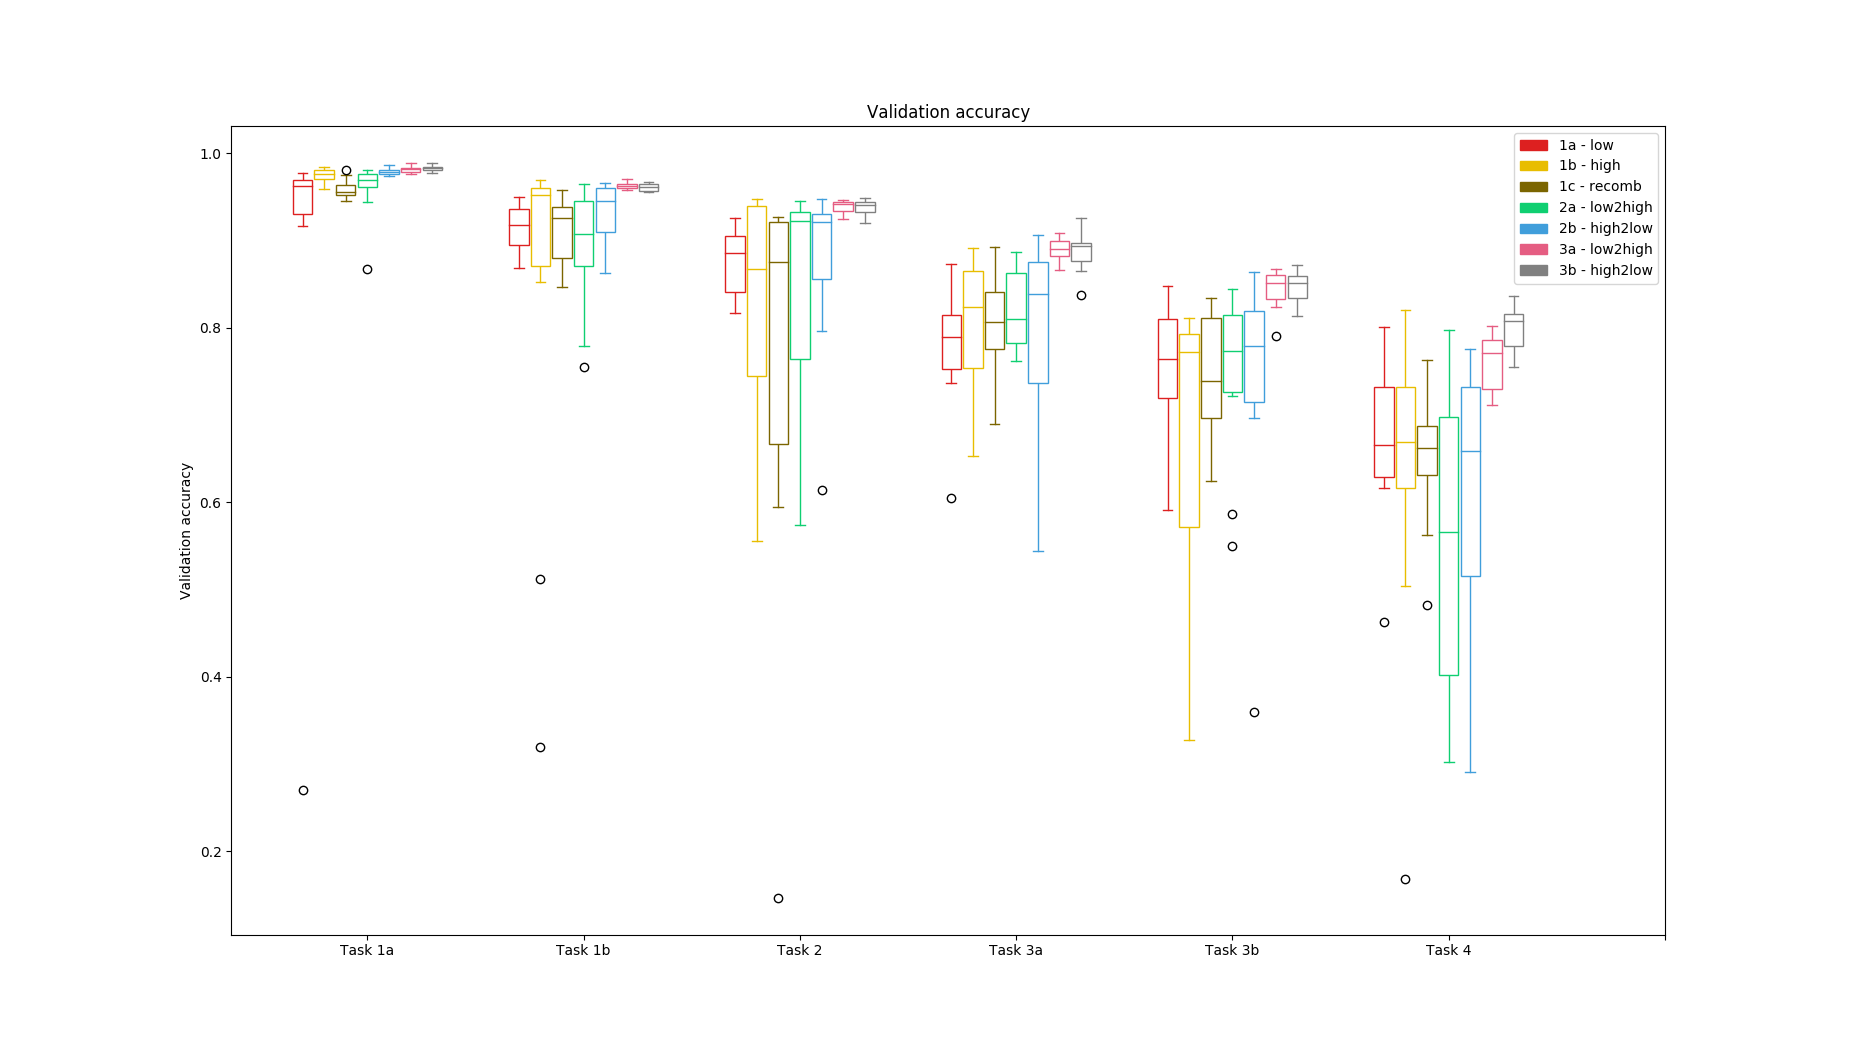
\includegraphics[width=\textwidth]{Chapters/Experiments/search_algo/figures/validation_boxplot.png}
    \caption{Boxplot of validation accuracy reached for each task and each algorithm.}
    \label{fig:search.validation}
\end{figure}

Across all metrics, 1a and 1c have about the same performance. An ANOVA test confirm there is no significant difference between the two algorithms validation accuracy means. Plot \ref{fig:search.training_value} shows algorithm 1c trains a bit more on average than 1a, but this is to be expected as the tournament size for algorithm 1c is three while 1a has the lowest size at two. 

During the searches, plot \ref{fig:search.avg_path_size} indicated algorithm 1c tends to yield larger paths on average than 1a, but a significance test of the average size of optimal paths for the two algorithms does not lend confidence to this claim. In fact, no significant difference were found between the average size of selected optimal paths or between the average path size in the final generation in each search, meaning the results shown in \ref{fig:search.avg_path_size} is not significant.

The diversity plots indicates that neither of the algorithms with low selection pressure reaches some state of converged population, where algorithm 1c barely changes. Measuring the diversity of this algorithm as a unique genome frequency does not work, as the recombination makes sure the next generations new genome is not a duplicate unless both parents are equal. The probability of the population having a significant portion being duplicates of each other is to low for this to have a decent chance of happening within the first 100 generations. 

\subsection{Scaling selection pressure}
Algorithms 2a and 2b does not differ in performance from each other or the algorithms with low selection pressure, and they do not have a significant difference for any metric other than module reuse. 

After task 3b, the mean reuse in the two algorithms were not significantly different and around 5, but for task 6 there is a jump of 1.5 modules on average. This is prominent in plot \ref{fig:search.reuse}. There is no obvious reason behind this jump except for the tournament size for this task, and a some ANOVA tests confirm that algorithms with a high tournament size of 25 for the last task have no significant difference in module reuse.  

Regarding convergence rate and diversity metrics, the two algorithms does not produce anything unexpected. Low tournament size leads to low convergence rate and vice versa, meaning both algorithms gradually change between high and low convergence rate depending on whether the algorithm increase or decrease tournament size for each task.

\subsection{Dynamic selection pressure}
The last two algorithms 3a and 3b gave the most consistent results for performance and resource demands. They both reach a higher classification accuracy on the validation data which differ significantly from the rest of the algorithms for all tasks on cSVHN. Between them the only performance difference is at the last task where algorithm 3b scores the highest of all algorithms tested with a mean classification accuracy of 80\%\footnote{In the original PathNet paper, a PathNet structure pretrained on the CIFAR set reached a classification accuracy of about 40\% after 500 generations when training on cSVHN, however the PathNet consisted of fully connected modules and not convolutional operations which is the case here.}.

The trade-off for the comparatively high classification accuracy comes in the amount of training where they train longer than the other algorithms with changing selection pressure (2a and 2b). Using multiple ANOVA tests, mean amount of training units of algorithm 3b does not differ from algorithm 1b, but 1b have a higher training mean than 3a.

Again by using multiple ANOVA tests, the amount of module reuse for algorithms 3a and 3b for task 4 can be shown to not differ from each other but have a lower reuse than all other algorithms. 

\subsection{High selection pressure}
Excluding algorithms 3a and 3b from an ANOVA test tells us there is no significant difference in validation accuracy means for any of the other algorithms, meaning algorithm 1b can not be shown to give better classification accuracy for all its extra training. 
In fact, excluding algorithm 3b which as mentioned undergo as much training, algorithm 1b has a significantly higher mean than every other algorithm and therefore also a much longer run-time. 

In metrics such as reuse and capacity use there is no difference between the algorithms with static selection pressure. 

\section{Conclusion}

The low selection pressure of algorithm 1c causes it to converge towards an optimal path to slowly in this experiment for any benefit from the high exploration rate to become visible. With a lower population size or a higher search termination limit the algorithm might reach a population with such a low diversity so that we could conclude it had found a path from an area of optimal fitness, but at that point the modules would most likely have overfitted to the training data. In a saturated PathNet the search problem is reduced from being a optimization of both weights and module selection to just module selection where no overfitting can occur\footnote{Theoretically, overfitting could take place in such a setting if we imagine the search space is populated with a vast number of optimal modules adapted to contain only small units of memetic knowledge, but this is an unrealistic scenario far from the structure of this PathNet implementation.}, but in that case, another optimization scheme might work better than tournament search. 

To a lesser extent this is true for algorithm 1a also, where it performs similarly to 1c in every metric except for diversity and convergence where the lower tournament size with no recombination has a higher selection pressure and therefore might reach a population state with an optimal path and mutations on that genotype.  

That being said, the performance of these algorithms is no different from those of high selection pressure and therefore high exploitation, so with regards to training time algorithm 1a and 1c is superior to the others where 1a seems to be the better choice. 

When performing ANOVA tests on the amount of module reuse, a test of the null hypothesis
\begin{equation*}
    H_{0}:\bar{\mu}_{1_{a}}=\bar{\mu}_{1_{b}}=\bar{\mu}_{1_{c}}=\bar{\mu}_{2_{b}}=\bar{\mu}_{3_{a}}
\end{equation*}
yields a P-value not sufficient to reject \(H_{0}\), while adding either 2a or 3b to the test causes \(H_{0}\) to be rejected. While this makes a case for high selection pressure leading to higher reuse, null hypothesis for \(\bar{\mu}_{2_{a}}=\bar{\mu}_{1_{b}}\) can not be rejected, but 2a and 2b is shown to be significantly different from each other. From this, the conclusion drawn is that more experimental runs are needed to be able to say anything meaningful about what causes an increase in module reuse.

With no change to accuracy but with 4 to 5 times the training amount over algorithms with low selection pressure, the static high tournament size of algorithm 1b is therefore concluded not to be well suited for this type of search. Algorithms 2a and 2b, while having a lower training amount than 1b, does also not improve on accuracy. 

Best performance is reached with algorithm 3a and 3b, where 3b reaches a higher accuracy for the last task. In plot \ref{fig:search.accuracy}, it looks like 3b is still improving when the search is terminated, hinting at the search termination limit might be to low for this algorithm also. The training amount for these algorithms is around the 9000 iterations mark, meaning the increase in accuracy comes by training significantly more. 

